%Przykładowy plik ułatwiający złożenie projektu dyplomowego inżynierskiego.
%UWAGA: Generowany napis na stronie tytułowej o treści PROJEKT DYPLOMOWY INŻYNIERSKI został zaproponowany przeze mnie i nie jest, póki co, potwierdzony przez władze wydziału. Przed ostatecznym oddaniem tak złożonej pracy należy upewnić się jaka powinna być treść tego napisu. W momencie gdy uzyskam informację na temat treści tego napisu, dokonam niezbędnych zmian w źródłach.

\documentclass[eng,printmode]{mgr}
%opcje klasy dokumentu mgr.cls zostały opisane w dołączonej instrukcji

%poniżej deklaracje użycia pakietów, usunąć to co jest niepotrzebne
\usepackage{polski} %przydatne podczas składania dokumentów w j. polskim
%\usepackage[polish]{babel}%alternatywnie do pakietu polski, wybrać jeden z nich
\usepackage[utf8]{inputenc} %kodowanie znaków, zależne od systemu
\usepackage[T1]{fontenc} %poprawne składanie polskich czcionek
\usepackage{qtree} %drzewa
\usepackage{hyperref} %hyperłącza
\usepackage{listings,xcolor} %jsony

%pakiety do grafiki
\usepackage{graphicx}
\usepackage{subfigure}
\usepackage{psfrag}

%pakiety dodające dużo dodatkowych poleceń matematycznych
\usepackage{amsmath}
\usepackage{amsfonts}

%pakiety wspomagające i poprawiające składanie tabel
\usepackage{supertabular}
\usepackage{array}
\usepackage{tabularx}
\usepackage{hhline}
\usepackage{pythonhighlight}

%pakiet wypisujący na marginesie etykiety równań i rysunków zdefiniowanych przez \label{}, chcąc wygenerować finalną wersję dokumentu wystarczy usunąć poniższą linię
\usepackage{showlabels}

 %%%%%%%%%%%%%%%%%%%%%%%%%%%%%%%%%%%%%%%%%%%%%%%%%%%%%%%%%%%%%%%%%%%%%%%%%%%%%%%% 
%%% ~ Arduino Language - Arduino IDE Colors ~                                  %%%
%%%                                                                            %%%
%%% Kyle Rocha-Brownell | 10/2/2017 | No Licence                               %%%
%%% -------------------------------------------------------------------------- %%%
%%%                                                                            %%%
%%% Place this file in your working directory (next to the latex file you're   %%%
%%% working on).  To add it to your project, place:                            %%%
%%%     %%%%%%%%%%%%%%%%%%%%%%%%%%%%%%%%%%%%%%%%%%%%%%%%%%%%%%%%%%%%%%%%%%%%%%%%%%%%%%%% 
%%% ~ Arduino Language - Arduino IDE Colors ~                                  %%%
%%%                                                                            %%%
%%% Kyle Rocha-Brownell | 10/2/2017 | No Licence                               %%%
%%% -------------------------------------------------------------------------- %%%
%%%                                                                            %%%
%%% Place this file in your working directory (next to the latex file you're   %%%
%%% working on).  To add it to your project, place:                            %%%
%%%     %%%%%%%%%%%%%%%%%%%%%%%%%%%%%%%%%%%%%%%%%%%%%%%%%%%%%%%%%%%%%%%%%%%%%%%%%%%%%%%% 
%%% ~ Arduino Language - Arduino IDE Colors ~                                  %%%
%%%                                                                            %%%
%%% Kyle Rocha-Brownell | 10/2/2017 | No Licence                               %%%
%%% -------------------------------------------------------------------------- %%%
%%%                                                                            %%%
%%% Place this file in your working directory (next to the latex file you're   %%%
%%% working on).  To add it to your project, place:                            %%%
%%%    \input{arduinoLanguage.tex}                                             %%%
%%% somewhere before \begin{document} in your latex file.                      %%%
%%%                                                                            %%%
%%% In your document, place your arduino code between:                         %%%
%%%   \begin{lstlisting}[language=Arduino]                                     %%%
%%% and:                                                                       %%%
%%%   \end{lstlisting}                                                         %%%
%%%                                                                            %%%
%%% Or create your own style to add non-built-in functions and variables.      %%%
%%%                                                                            %%%
 %%%%%%%%%%%%%%%%%%%%%%%%%%%%%%%%%%%%%%%%%%%%%%%%%%%%%%%%%%%%%%%%%%%%%%%%%%%%%%%% 

\usepackage{color}
\usepackage{listings}    
\usepackage{courier}

%%% Define Custom IDE Colors %%%
\definecolor{arduinoGreen}    {rgb} {0.17, 0.43, 0.01}
\definecolor{arduinoGrey}     {rgb} {0.47, 0.47, 0.33}
\definecolor{arduinoOrange}   {rgb} {0.8 , 0.4 , 0   }
\definecolor{arduinoBlue}     {rgb} {0.01, 0.61, 0.98}
\definecolor{arduinoDarkBlue} {rgb} {0.0 , 0.2 , 0.5 }

%%% Define Arduino Language %%%
\lstdefinelanguage{Arduino}{
  language=C++, % begin with default C++ settings 
%
%
  %%% Keyword Color Group 1 %%%  (called KEYWORD3 by arduino)
  keywordstyle=\color{arduinoGreen},   
  deletekeywords={  % remove all arduino keywords that might be in c++
                break, case, override, final, continue, default, do, else, for, 
                if, return, goto, switch, throw, try, while, setup, loop, export, 
                not, or, and, xor, include, define, elif, else, error, if, ifdef, 
                ifndef, pragma, warning,
                HIGH, LOW, INPUT, INPUT_PULLUP, OUTPUT, DEC, BIN, HEX, OCT, PI, 
                HALF_PI, TWO_PI, LSBFIRST, MSBFIRST, CHANGE, FALLING, RISING, 
                DEFAULT, EXTERNAL, INTERNAL, INTERNAL1V1, INTERNAL2V56, LED_BUILTIN, 
                LED_BUILTIN_RX, LED_BUILTIN_TX, DIGITAL_MESSAGE, FIRMATA_STRING, 
                ANALOG_MESSAGE, REPORT_DIGITAL, REPORT_ANALOG, SET_PIN_MODE, 
                SYSTEM_RESET, SYSEX_START, auto, int8_t, int16_t, int32_t, int64_t, 
                uint8_t, uint16_t, uint32_t, uint64_t, char16_t, char32_t, operator, 
                enum, delete, bool, boolean, byte, char, const, false, float, double, 
                null, NULL, int, long, new, private, protected, public, short, 
                signed, static, volatile, String, void, true, unsigned, word, array, 
                sizeof, dynamic_cast, typedef, const_cast, struct, static_cast, union, 
                friend, extern, class, reinterpret_cast, register, explicit, inline, 
                _Bool, complex, _Complex, _Imaginary, atomic_bool, atomic_char, 
                atomic_schar, atomic_uchar, atomic_short, atomic_ushort, atomic_int, 
                atomic_uint, atomic_long, atomic_ulong, atomic_llong, atomic_ullong, 
                virtual, PROGMEM,
                Serial, Serial1, Serial2, Serial3, SerialUSB, Keyboard, Mouse,
                abs, acos, asin, atan, atan2, ceil, constrain, cos, degrees, exp, 
                floor, log, map, max, min, radians, random, randomSeed, round, sin, 
                sq, sqrt, tan, pow, bitRead, bitWrite, bitSet, bitClear, bit, 
                highByte, lowByte, analogReference, analogRead, 
                analogReadResolution, analogWrite, analogWriteResolution, 
                attachInterrupt, detachInterrupt, digitalPinToInterrupt, delay, 
                delayMicroseconds, digitalWrite, digitalRead, interrupts, millis, 
                micros, noInterrupts, noTone, pinMode, pulseIn, pulseInLong, shiftIn, 
                shiftOut, tone, yield, Stream, begin, end, peek, read, print, 
                println, available, availableForWrite, flush, setTimeout, find, 
                findUntil, parseInt, parseFloat, readBytes, readBytesUntil, readString, 
                readStringUntil, trim, toUpperCase, toLowerCase, charAt, compareTo, 
                concat, endsWith, startsWith, equals, equalsIgnoreCase, getBytes, 
                indexOf, lastIndexOf, length, replace, setCharAt, substring, 
                toCharArray, toInt, press, release, releaseAll, accept, click, move, 
                isPressed, isAlphaNumeric, isAlpha, isAscii, isWhitespace, isControl, 
                isDigit, isGraph, isLowerCase, isPrintable, isPunct, isSpace, 
                isUpperCase, isHexadecimalDigit, 
                }, 
  morekeywords={   % add arduino structures to group 1
                break, case, override, final, continue, default, do, else, for, 
                if, return, goto, switch, throw, try, while, setup, loop, export, 
                not, or, and, xor, include, define, elif, else, error, if, ifdef, 
                ifndef, pragma, warning,
                }, 
% 
%
  %%% Keyword Color Group 2 %%%  (called LITERAL1 by arduino)
  keywordstyle=[2]\color{arduinoBlue},   
  keywords=[2]{   % add variables and dataTypes as 2nd group  
                HIGH, LOW, INPUT, INPUT_PULLUP, OUTPUT, DEC, BIN, HEX, OCT, PI, 
                HALF_PI, TWO_PI, LSBFIRST, MSBFIRST, CHANGE, FALLING, RISING, 
                DEFAULT, EXTERNAL, INTERNAL, INTERNAL1V1, INTERNAL2V56, LED_BUILTIN, 
                LED_BUILTIN_RX, LED_BUILTIN_TX, DIGITAL_MESSAGE, FIRMATA_STRING, 
                ANALOG_MESSAGE, REPORT_DIGITAL, REPORT_ANALOG, SET_PIN_MODE, 
                SYSTEM_RESET, SYSEX_START, auto, int8_t, int16_t, int32_t, int64_t, 
                uint8_t, uint16_t, uint32_t, uint64_t, char16_t, char32_t, operator, 
                enum, delete, bool, boolean, byte, char, const, false, float, double, 
                null, NULL, int, long, new, private, protected, public, short, 
                signed, static, volatile, String, void, true, unsigned, word, array, 
                sizeof, dynamic_cast, typedef, const_cast, struct, static_cast, union, 
                friend, extern, class, reinterpret_cast, register, explicit, inline, 
                _Bool, complex, _Complex, _Imaginary, atomic_bool, atomic_char, 
                atomic_schar, atomic_uchar, atomic_short, atomic_ushort, atomic_int, 
                atomic_uint, atomic_long, atomic_ulong, atomic_llong, atomic_ullong, 
                virtual, PROGMEM,
                },  
% 
%
  %%% Keyword Color Group 3 %%%  (called KEYWORD1 by arduino)
  keywordstyle=[3]\bfseries\color{arduinoOrange},
  keywords=[3]{  % add built-in functions as a 3rd group
                Serial, Serial1, Serial2, Serial3, SerialUSB, Keyboard, Mouse,
                },      
%
%
  %%% Keyword Color Group 4 %%%  (called KEYWORD2 by arduino)
  keywordstyle=[4]\color{arduinoOrange},
  keywords=[4]{  % add more built-in functions as a 4th group
                abs, acos, asin, atan, atan2, ceil, constrain, cos, degrees, exp, 
                floor, log, map, max, min, radians, random, randomSeed, round, sin, 
                sq, sqrt, tan, pow, bitRead, bitWrite, bitSet, bitClear, bit, 
                highByte, lowByte, analogReference, analogRead, 
                analogReadResolution, analogWrite, analogWriteResolution, 
                attachInterrupt, detachInterrupt, digitalPinToInterrupt, delay, 
                delayMicroseconds, digitalWrite, digitalRead, interrupts, millis, 
                micros, noInterrupts, noTone, pinMode, pulseIn, pulseInLong, shiftIn, 
                shiftOut, tone, yield, Stream, begin, end, peek, read, print, 
                println, available, availableForWrite, flush, setTimeout, find, 
                findUntil, parseInt, parseFloat, readBytes, readBytesUntil, readString, 
                readStringUntil, trim, toUpperCase, toLowerCase, charAt, compareTo, 
                concat, endsWith, startsWith, equals, equalsIgnoreCase, getBytes, 
                indexOf, lastIndexOf, length, replace, setCharAt, substring, 
                toCharArray, toInt, press, release, releaseAll, accept, click, move, 
                isPressed, isAlphaNumeric, isAlpha, isAscii, isWhitespace, isControl, 
                isDigit, isGraph, isLowerCase, isPrintable, isPunct, isSpace, 
                isUpperCase, isHexadecimalDigit, 
                },      
%
%
  %%% Set Other Colors %%%
  stringstyle=\color{arduinoDarkBlue},    
  commentstyle=\color{arduinoGrey},    
%          
%   
  %%%% Line Numbering %%%%
   numbers=left,                    
  numbersep=5pt,                   
  numberstyle=\color{arduinoGrey},    
  %stepnumber=2,                      % show every 2 line numbers
%
%
  %%%% Code Box Style %%%%
  breaklines=true,                    % wordwrapping
  tabsize=2,         
  basicstyle=\ttfamily  
}                                             %%%
%%% somewhere before \begin{document} in your latex file.                      %%%
%%%                                                                            %%%
%%% In your document, place your arduino code between:                         %%%
%%%   \begin{lstlisting}[language=Arduino]                                     %%%
%%% and:                                                                       %%%
%%%   \end{lstlisting}                                                         %%%
%%%                                                                            %%%
%%% Or create your own style to add non-built-in functions and variables.      %%%
%%%                                                                            %%%
 %%%%%%%%%%%%%%%%%%%%%%%%%%%%%%%%%%%%%%%%%%%%%%%%%%%%%%%%%%%%%%%%%%%%%%%%%%%%%%%% 

\usepackage{color}
\usepackage{listings}    
\usepackage{courier}

%%% Define Custom IDE Colors %%%
\definecolor{arduinoGreen}    {rgb} {0.17, 0.43, 0.01}
\definecolor{arduinoGrey}     {rgb} {0.47, 0.47, 0.33}
\definecolor{arduinoOrange}   {rgb} {0.8 , 0.4 , 0   }
\definecolor{arduinoBlue}     {rgb} {0.01, 0.61, 0.98}
\definecolor{arduinoDarkBlue} {rgb} {0.0 , 0.2 , 0.5 }

%%% Define Arduino Language %%%
\lstdefinelanguage{Arduino}{
  language=C++, % begin with default C++ settings 
%
%
  %%% Keyword Color Group 1 %%%  (called KEYWORD3 by arduino)
  keywordstyle=\color{arduinoGreen},   
  deletekeywords={  % remove all arduino keywords that might be in c++
                break, case, override, final, continue, default, do, else, for, 
                if, return, goto, switch, throw, try, while, setup, loop, export, 
                not, or, and, xor, include, define, elif, else, error, if, ifdef, 
                ifndef, pragma, warning,
                HIGH, LOW, INPUT, INPUT_PULLUP, OUTPUT, DEC, BIN, HEX, OCT, PI, 
                HALF_PI, TWO_PI, LSBFIRST, MSBFIRST, CHANGE, FALLING, RISING, 
                DEFAULT, EXTERNAL, INTERNAL, INTERNAL1V1, INTERNAL2V56, LED_BUILTIN, 
                LED_BUILTIN_RX, LED_BUILTIN_TX, DIGITAL_MESSAGE, FIRMATA_STRING, 
                ANALOG_MESSAGE, REPORT_DIGITAL, REPORT_ANALOG, SET_PIN_MODE, 
                SYSTEM_RESET, SYSEX_START, auto, int8_t, int16_t, int32_t, int64_t, 
                uint8_t, uint16_t, uint32_t, uint64_t, char16_t, char32_t, operator, 
                enum, delete, bool, boolean, byte, char, const, false, float, double, 
                null, NULL, int, long, new, private, protected, public, short, 
                signed, static, volatile, String, void, true, unsigned, word, array, 
                sizeof, dynamic_cast, typedef, const_cast, struct, static_cast, union, 
                friend, extern, class, reinterpret_cast, register, explicit, inline, 
                _Bool, complex, _Complex, _Imaginary, atomic_bool, atomic_char, 
                atomic_schar, atomic_uchar, atomic_short, atomic_ushort, atomic_int, 
                atomic_uint, atomic_long, atomic_ulong, atomic_llong, atomic_ullong, 
                virtual, PROGMEM,
                Serial, Serial1, Serial2, Serial3, SerialUSB, Keyboard, Mouse,
                abs, acos, asin, atan, atan2, ceil, constrain, cos, degrees, exp, 
                floor, log, map, max, min, radians, random, randomSeed, round, sin, 
                sq, sqrt, tan, pow, bitRead, bitWrite, bitSet, bitClear, bit, 
                highByte, lowByte, analogReference, analogRead, 
                analogReadResolution, analogWrite, analogWriteResolution, 
                attachInterrupt, detachInterrupt, digitalPinToInterrupt, delay, 
                delayMicroseconds, digitalWrite, digitalRead, interrupts, millis, 
                micros, noInterrupts, noTone, pinMode, pulseIn, pulseInLong, shiftIn, 
                shiftOut, tone, yield, Stream, begin, end, peek, read, print, 
                println, available, availableForWrite, flush, setTimeout, find, 
                findUntil, parseInt, parseFloat, readBytes, readBytesUntil, readString, 
                readStringUntil, trim, toUpperCase, toLowerCase, charAt, compareTo, 
                concat, endsWith, startsWith, equals, equalsIgnoreCase, getBytes, 
                indexOf, lastIndexOf, length, replace, setCharAt, substring, 
                toCharArray, toInt, press, release, releaseAll, accept, click, move, 
                isPressed, isAlphaNumeric, isAlpha, isAscii, isWhitespace, isControl, 
                isDigit, isGraph, isLowerCase, isPrintable, isPunct, isSpace, 
                isUpperCase, isHexadecimalDigit, 
                }, 
  morekeywords={   % add arduino structures to group 1
                break, case, override, final, continue, default, do, else, for, 
                if, return, goto, switch, throw, try, while, setup, loop, export, 
                not, or, and, xor, include, define, elif, else, error, if, ifdef, 
                ifndef, pragma, warning,
                }, 
% 
%
  %%% Keyword Color Group 2 %%%  (called LITERAL1 by arduino)
  keywordstyle=[2]\color{arduinoBlue},   
  keywords=[2]{   % add variables and dataTypes as 2nd group  
                HIGH, LOW, INPUT, INPUT_PULLUP, OUTPUT, DEC, BIN, HEX, OCT, PI, 
                HALF_PI, TWO_PI, LSBFIRST, MSBFIRST, CHANGE, FALLING, RISING, 
                DEFAULT, EXTERNAL, INTERNAL, INTERNAL1V1, INTERNAL2V56, LED_BUILTIN, 
                LED_BUILTIN_RX, LED_BUILTIN_TX, DIGITAL_MESSAGE, FIRMATA_STRING, 
                ANALOG_MESSAGE, REPORT_DIGITAL, REPORT_ANALOG, SET_PIN_MODE, 
                SYSTEM_RESET, SYSEX_START, auto, int8_t, int16_t, int32_t, int64_t, 
                uint8_t, uint16_t, uint32_t, uint64_t, char16_t, char32_t, operator, 
                enum, delete, bool, boolean, byte, char, const, false, float, double, 
                null, NULL, int, long, new, private, protected, public, short, 
                signed, static, volatile, String, void, true, unsigned, word, array, 
                sizeof, dynamic_cast, typedef, const_cast, struct, static_cast, union, 
                friend, extern, class, reinterpret_cast, register, explicit, inline, 
                _Bool, complex, _Complex, _Imaginary, atomic_bool, atomic_char, 
                atomic_schar, atomic_uchar, atomic_short, atomic_ushort, atomic_int, 
                atomic_uint, atomic_long, atomic_ulong, atomic_llong, atomic_ullong, 
                virtual, PROGMEM,
                },  
% 
%
  %%% Keyword Color Group 3 %%%  (called KEYWORD1 by arduino)
  keywordstyle=[3]\bfseries\color{arduinoOrange},
  keywords=[3]{  % add built-in functions as a 3rd group
                Serial, Serial1, Serial2, Serial3, SerialUSB, Keyboard, Mouse,
                },      
%
%
  %%% Keyword Color Group 4 %%%  (called KEYWORD2 by arduino)
  keywordstyle=[4]\color{arduinoOrange},
  keywords=[4]{  % add more built-in functions as a 4th group
                abs, acos, asin, atan, atan2, ceil, constrain, cos, degrees, exp, 
                floor, log, map, max, min, radians, random, randomSeed, round, sin, 
                sq, sqrt, tan, pow, bitRead, bitWrite, bitSet, bitClear, bit, 
                highByte, lowByte, analogReference, analogRead, 
                analogReadResolution, analogWrite, analogWriteResolution, 
                attachInterrupt, detachInterrupt, digitalPinToInterrupt, delay, 
                delayMicroseconds, digitalWrite, digitalRead, interrupts, millis, 
                micros, noInterrupts, noTone, pinMode, pulseIn, pulseInLong, shiftIn, 
                shiftOut, tone, yield, Stream, begin, end, peek, read, print, 
                println, available, availableForWrite, flush, setTimeout, find, 
                findUntil, parseInt, parseFloat, readBytes, readBytesUntil, readString, 
                readStringUntil, trim, toUpperCase, toLowerCase, charAt, compareTo, 
                concat, endsWith, startsWith, equals, equalsIgnoreCase, getBytes, 
                indexOf, lastIndexOf, length, replace, setCharAt, substring, 
                toCharArray, toInt, press, release, releaseAll, accept, click, move, 
                isPressed, isAlphaNumeric, isAlpha, isAscii, isWhitespace, isControl, 
                isDigit, isGraph, isLowerCase, isPrintable, isPunct, isSpace, 
                isUpperCase, isHexadecimalDigit, 
                },      
%
%
  %%% Set Other Colors %%%
  stringstyle=\color{arduinoDarkBlue},    
  commentstyle=\color{arduinoGrey},    
%          
%   
  %%%% Line Numbering %%%%
   numbers=left,                    
  numbersep=5pt,                   
  numberstyle=\color{arduinoGrey},    
  %stepnumber=2,                      % show every 2 line numbers
%
%
  %%%% Code Box Style %%%%
  breaklines=true,                    % wordwrapping
  tabsize=2,         
  basicstyle=\ttfamily  
}                                             %%%
%%% somewhere before \begin{document} in your latex file.                      %%%
%%%                                                                            %%%
%%% In your document, place your arduino code between:                         %%%
%%%   \begin{lstlisting}[language=Arduino]                                     %%%
%%% and:                                                                       %%%
%%%   \end{lstlisting}                                                         %%%
%%%                                                                            %%%
%%% Or create your own style to add non-built-in functions and variables.      %%%
%%%                                                                            %%%
 %%%%%%%%%%%%%%%%%%%%%%%%%%%%%%%%%%%%%%%%%%%%%%%%%%%%%%%%%%%%%%%%%%%%%%%%%%%%%%%% 

\usepackage{color}
\usepackage{listings}    
\usepackage{courier}

%%% Define Custom IDE Colors %%%
\definecolor{arduinoGreen}    {rgb} {0.17, 0.43, 0.01}
\definecolor{arduinoGrey}     {rgb} {0.47, 0.47, 0.33}
\definecolor{arduinoOrange}   {rgb} {0.8 , 0.4 , 0   }
\definecolor{arduinoBlue}     {rgb} {0.01, 0.61, 0.98}
\definecolor{arduinoDarkBlue} {rgb} {0.0 , 0.2 , 0.5 }

%%% Define Arduino Language %%%
\lstdefinelanguage{Arduino}{
  language=C++, % begin with default C++ settings 
%
%
  %%% Keyword Color Group 1 %%%  (called KEYWORD3 by arduino)
  keywordstyle=\color{arduinoGreen},   
  deletekeywords={  % remove all arduino keywords that might be in c++
                break, case, override, final, continue, default, do, else, for, 
                if, return, goto, switch, throw, try, while, setup, loop, export, 
                not, or, and, xor, include, define, elif, else, error, if, ifdef, 
                ifndef, pragma, warning,
                HIGH, LOW, INPUT, INPUT_PULLUP, OUTPUT, DEC, BIN, HEX, OCT, PI, 
                HALF_PI, TWO_PI, LSBFIRST, MSBFIRST, CHANGE, FALLING, RISING, 
                DEFAULT, EXTERNAL, INTERNAL, INTERNAL1V1, INTERNAL2V56, LED_BUILTIN, 
                LED_BUILTIN_RX, LED_BUILTIN_TX, DIGITAL_MESSAGE, FIRMATA_STRING, 
                ANALOG_MESSAGE, REPORT_DIGITAL, REPORT_ANALOG, SET_PIN_MODE, 
                SYSTEM_RESET, SYSEX_START, auto, int8_t, int16_t, int32_t, int64_t, 
                uint8_t, uint16_t, uint32_t, uint64_t, char16_t, char32_t, operator, 
                enum, delete, bool, boolean, byte, char, const, false, float, double, 
                null, NULL, int, long, new, private, protected, public, short, 
                signed, static, volatile, String, void, true, unsigned, word, array, 
                sizeof, dynamic_cast, typedef, const_cast, struct, static_cast, union, 
                friend, extern, class, reinterpret_cast, register, explicit, inline, 
                _Bool, complex, _Complex, _Imaginary, atomic_bool, atomic_char, 
                atomic_schar, atomic_uchar, atomic_short, atomic_ushort, atomic_int, 
                atomic_uint, atomic_long, atomic_ulong, atomic_llong, atomic_ullong, 
                virtual, PROGMEM,
                Serial, Serial1, Serial2, Serial3, SerialUSB, Keyboard, Mouse,
                abs, acos, asin, atan, atan2, ceil, constrain, cos, degrees, exp, 
                floor, log, map, max, min, radians, random, randomSeed, round, sin, 
                sq, sqrt, tan, pow, bitRead, bitWrite, bitSet, bitClear, bit, 
                highByte, lowByte, analogReference, analogRead, 
                analogReadResolution, analogWrite, analogWriteResolution, 
                attachInterrupt, detachInterrupt, digitalPinToInterrupt, delay, 
                delayMicroseconds, digitalWrite, digitalRead, interrupts, millis, 
                micros, noInterrupts, noTone, pinMode, pulseIn, pulseInLong, shiftIn, 
                shiftOut, tone, yield, Stream, begin, end, peek, read, print, 
                println, available, availableForWrite, flush, setTimeout, find, 
                findUntil, parseInt, parseFloat, readBytes, readBytesUntil, readString, 
                readStringUntil, trim, toUpperCase, toLowerCase, charAt, compareTo, 
                concat, endsWith, startsWith, equals, equalsIgnoreCase, getBytes, 
                indexOf, lastIndexOf, length, replace, setCharAt, substring, 
                toCharArray, toInt, press, release, releaseAll, accept, click, move, 
                isPressed, isAlphaNumeric, isAlpha, isAscii, isWhitespace, isControl, 
                isDigit, isGraph, isLowerCase, isPrintable, isPunct, isSpace, 
                isUpperCase, isHexadecimalDigit, 
                }, 
  morekeywords={   % add arduino structures to group 1
                break, case, override, final, continue, default, do, else, for, 
                if, return, goto, switch, throw, try, while, setup, loop, export, 
                not, or, and, xor, include, define, elif, else, error, if, ifdef, 
                ifndef, pragma, warning,
                }, 
% 
%
  %%% Keyword Color Group 2 %%%  (called LITERAL1 by arduino)
  keywordstyle=[2]\color{arduinoBlue},   
  keywords=[2]{   % add variables and dataTypes as 2nd group  
                HIGH, LOW, INPUT, INPUT_PULLUP, OUTPUT, DEC, BIN, HEX, OCT, PI, 
                HALF_PI, TWO_PI, LSBFIRST, MSBFIRST, CHANGE, FALLING, RISING, 
                DEFAULT, EXTERNAL, INTERNAL, INTERNAL1V1, INTERNAL2V56, LED_BUILTIN, 
                LED_BUILTIN_RX, LED_BUILTIN_TX, DIGITAL_MESSAGE, FIRMATA_STRING, 
                ANALOG_MESSAGE, REPORT_DIGITAL, REPORT_ANALOG, SET_PIN_MODE, 
                SYSTEM_RESET, SYSEX_START, auto, int8_t, int16_t, int32_t, int64_t, 
                uint8_t, uint16_t, uint32_t, uint64_t, char16_t, char32_t, operator, 
                enum, delete, bool, boolean, byte, char, const, false, float, double, 
                null, NULL, int, long, new, private, protected, public, short, 
                signed, static, volatile, String, void, true, unsigned, word, array, 
                sizeof, dynamic_cast, typedef, const_cast, struct, static_cast, union, 
                friend, extern, class, reinterpret_cast, register, explicit, inline, 
                _Bool, complex, _Complex, _Imaginary, atomic_bool, atomic_char, 
                atomic_schar, atomic_uchar, atomic_short, atomic_ushort, atomic_int, 
                atomic_uint, atomic_long, atomic_ulong, atomic_llong, atomic_ullong, 
                virtual, PROGMEM,
                },  
% 
%
  %%% Keyword Color Group 3 %%%  (called KEYWORD1 by arduino)
  keywordstyle=[3]\bfseries\color{arduinoOrange},
  keywords=[3]{  % add built-in functions as a 3rd group
                Serial, Serial1, Serial2, Serial3, SerialUSB, Keyboard, Mouse,
                },      
%
%
  %%% Keyword Color Group 4 %%%  (called KEYWORD2 by arduino)
  keywordstyle=[4]\color{arduinoOrange},
  keywords=[4]{  % add more built-in functions as a 4th group
                abs, acos, asin, atan, atan2, ceil, constrain, cos, degrees, exp, 
                floor, log, map, max, min, radians, random, randomSeed, round, sin, 
                sq, sqrt, tan, pow, bitRead, bitWrite, bitSet, bitClear, bit, 
                highByte, lowByte, analogReference, analogRead, 
                analogReadResolution, analogWrite, analogWriteResolution, 
                attachInterrupt, detachInterrupt, digitalPinToInterrupt, delay, 
                delayMicroseconds, digitalWrite, digitalRead, interrupts, millis, 
                micros, noInterrupts, noTone, pinMode, pulseIn, pulseInLong, shiftIn, 
                shiftOut, tone, yield, Stream, begin, end, peek, read, print, 
                println, available, availableForWrite, flush, setTimeout, find, 
                findUntil, parseInt, parseFloat, readBytes, readBytesUntil, readString, 
                readStringUntil, trim, toUpperCase, toLowerCase, charAt, compareTo, 
                concat, endsWith, startsWith, equals, equalsIgnoreCase, getBytes, 
                indexOf, lastIndexOf, length, replace, setCharAt, substring, 
                toCharArray, toInt, press, release, releaseAll, accept, click, move, 
                isPressed, isAlphaNumeric, isAlpha, isAscii, isWhitespace, isControl, 
                isDigit, isGraph, isLowerCase, isPrintable, isPunct, isSpace, 
                isUpperCase, isHexadecimalDigit, 
                },      
%
%
  %%% Set Other Colors %%%
  stringstyle=\color{arduinoDarkBlue},    
  commentstyle=\color{arduinoGrey},    
%          
%   
  %%%% Line Numbering %%%%
   numbers=left,                    
  numbersep=5pt,                   
  numberstyle=\color{arduinoGrey},    
  %stepnumber=2,                      % show every 2 line numbers
%
%
  %%%% Code Box Style %%%%
  breaklines=true,                    % wordwrapping
  tabsize=2,         
  basicstyle=\ttfamily  
}

%definicje własnych poleceń
\newcommand{\R}{I\!\!R} %symbol liczb rzeczywistych, działa tylko w trybie matematycznym
\newtheorem{theorem}{Twierdzenie}[section] %nowe otoczenie do składania twierdzeń
\graphicspath{ {./images/} }


%dane do złożenia strony tytułowej
\title{Projekt i realizacja urządzenia do zdalnej kontroli wzmacniacza gitarowego}
\engtitle{Design and implementation of a device for remote control of a guitar amplifier}
\author{Oleksii Pilkevych}
\supervisor{dr inż. Paweł Ksieniewicz PWr}
%\guardian{dr hab. inż. Imię Nazwisko Prof. PWr, I-6} %nie używać jeśli opiekun jest tą samą osobą co prowadzący pracę

\date{2019} %standardowo u dołu strony tytułowej umieszczany jest bieżący rok, to polecenie pozwala wstawić dowolny rok

%poniżej jest lista kierunków i specjalności na wydziale elektroniki, należy wybrać właściwe lub dopisać jeśli nie ma odpowiednich
\field{Informatyka (INF)}
\specialisation{Inżynieria internetowa (INT)}

%tutaj zaczyna się właściwa treść dokumentu
\begin{document}
\bibliographystyle{plabbrv} %tylko gdy używamy BibTeXa, ustawia polski styl bibliografii

\maketitle %polecenie generujące stronę tytułową
% \dedication{6cm}{To jest przykładowa treść opcjonalnej dedykacji, należy ją zmienić lub usunąć w całości polecenie \texttt{$\backslash$dedication}}

\tableofcontents %spis treści

%poniżej znajduje się przykładowa treść dalszej części dokumentu, zainteresowanych zachęcam do rozszyfrowania frazy "Lorem ipsum" :)
\chapter{Wstęp}
\section{Motywacja}

Tematem pracy jest implementacja urządzenia do zdalnej kontroli wzmacniacza gitarowego. Mimo, że są rozpowszechnione systemy bezprzewodowe do przesyłania sygnału analogowego z przetworników gitary do wzmacniacza, nadal jest potrzeba przełączania "preset-ów" (ustawień) na wzmacniaczach podczas występów na żywo. Do tego zazwyczaj są używane przełączniki nożne, które są podpięte kablem do wzmacniacza i leżą na podłodze. Minusem tego rozwiązania, jest to, że gitarzysta powinien pamiętać kiedy ma wrócić do konkretnego miejsca na scenie w celu przełączenia na przykład czystego dźwięku na przesterowany.

Proponowanym przez tą pracę rozwiązaniem jest montaż urządzenia bezprzewodowego bezpośrednio na gitarze, co umożliwia wysyłanie dowolnych komunikatów MIDI zdalnie z dowolnego miejsca na scenie (w zasięgu urządzenia bezprzewodowego).
Komunikaty trafiają do odbiornika, który jest zasilany z gniazdka, albo power banku i jest podpięty kablem do wzmacniacza gitarowego.
Ponieważ protokół MIDI jest bardzo rozbudowany i uniwersalnie wspierane - daje to dużo większe możliwości niż samo przełączanie ustawień.

\section{Wymagania}

\begin{itemize}
\item Minimalny zasięg około 10 metrów
\item Mały pobór mocy nadajnika pozwalający na wykorzystanie baterii CR2032
\item Możliwość konfigurowania sekwencji komunikatów MIDI pod każdym przyciskiem
\item Czas reakcji nie większy niż 500 milisekund
\item Komunikacja odbiornika z wzmacniaczem przez interfejs MIDI (5-pinowe złącze DIN)
\end{itemize}

\section{Konkurencyjne rozwiązania}
\subsection{ACPAD}
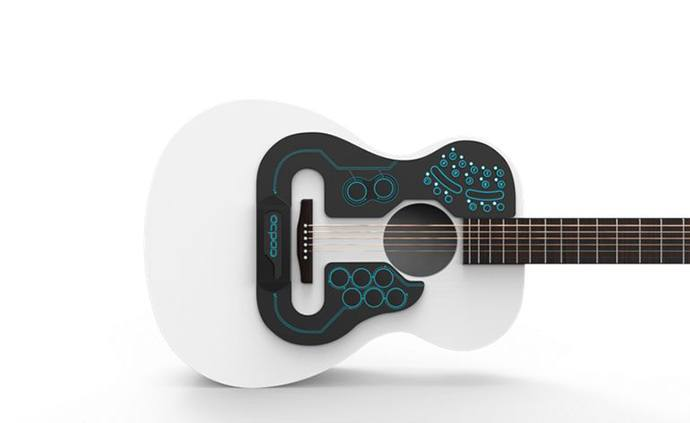
\includegraphics[width=\textwidth]{acpad}

ACPAD pojawił się na stronie Kickstarter w 2016 roku. Urządzenie jest skierowane wyłącznie na gitary akustyczne, ma wiele czujników piezoelektrycznych. Umożliwia zaprogramowanie różnych dźwięków pod każdy czujnik.

Mimo, że ACPAD był stworzony w celu umożliwienia grania na syntezatorach/wirtualnej perkusji podczas grania na gitarze akustycznej - ponieważ wspiera MIDI, jest możliwe również przełączanie ustawień.

Minusy:
\begin{itemize}
\item Wspiera wyłącznie gitary akustyczne
\item Jest dużo bardziej rozbudowane niż zwykły przełącznik ustawień, co powoduje, że więcej kosztuje (około 450 euro)
\item Nie ma odbiornika ze złączem MIDI tylko USB
\end{itemize}

\subsection{Livid Guitar Wing}
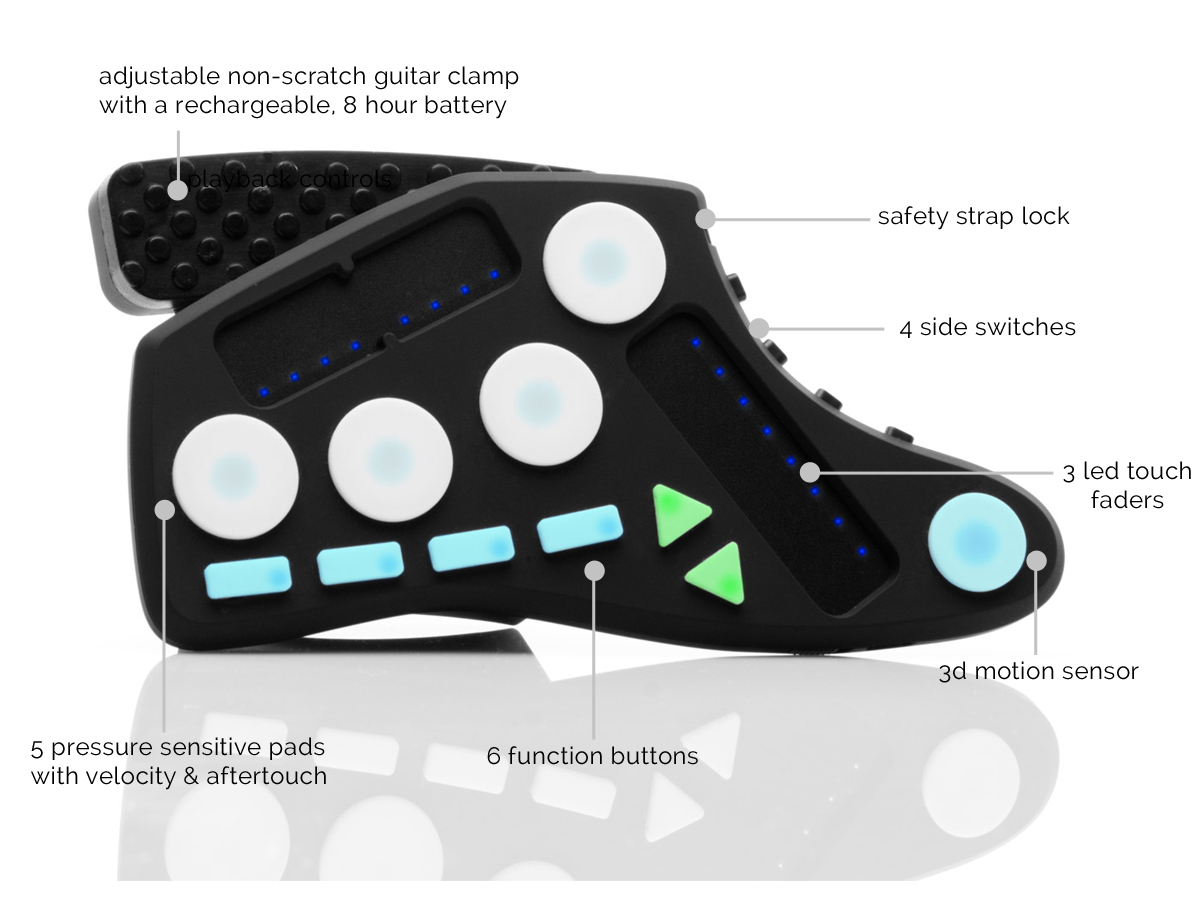
\includegraphics[width=\textwidth]{livid1}
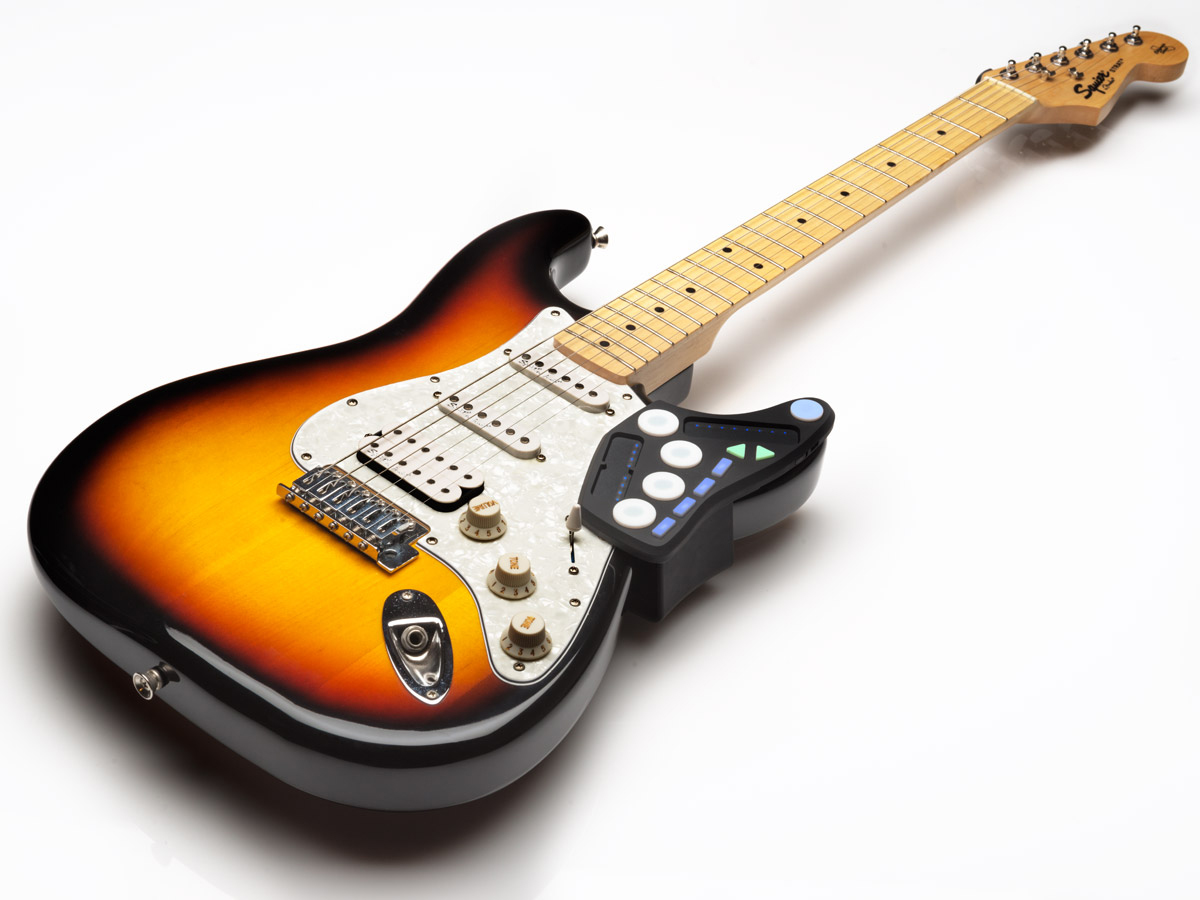
\includegraphics[width=\textwidth]{livid2}

Urządzenie jest oparte o Bluetooth low energy. Ma wiele czujników, przystępną cenę (130 dolarów).
Minusy:

\begin{itemize}
\item Jest zaprojektowane pod jedną specyficzną formę gitary
\item Nie ma odbiornika ze złączem MIDI, więc do przekierowania komunikatów MIDI do wzmacniacza byłby potrzebny laptop z zewnętrzną kartą dźwiękową, co utrudnia sprawę oraz wydłuża czas reakcji
\end{itemize}


\subsection{Aalberg audio MOON MO-1}
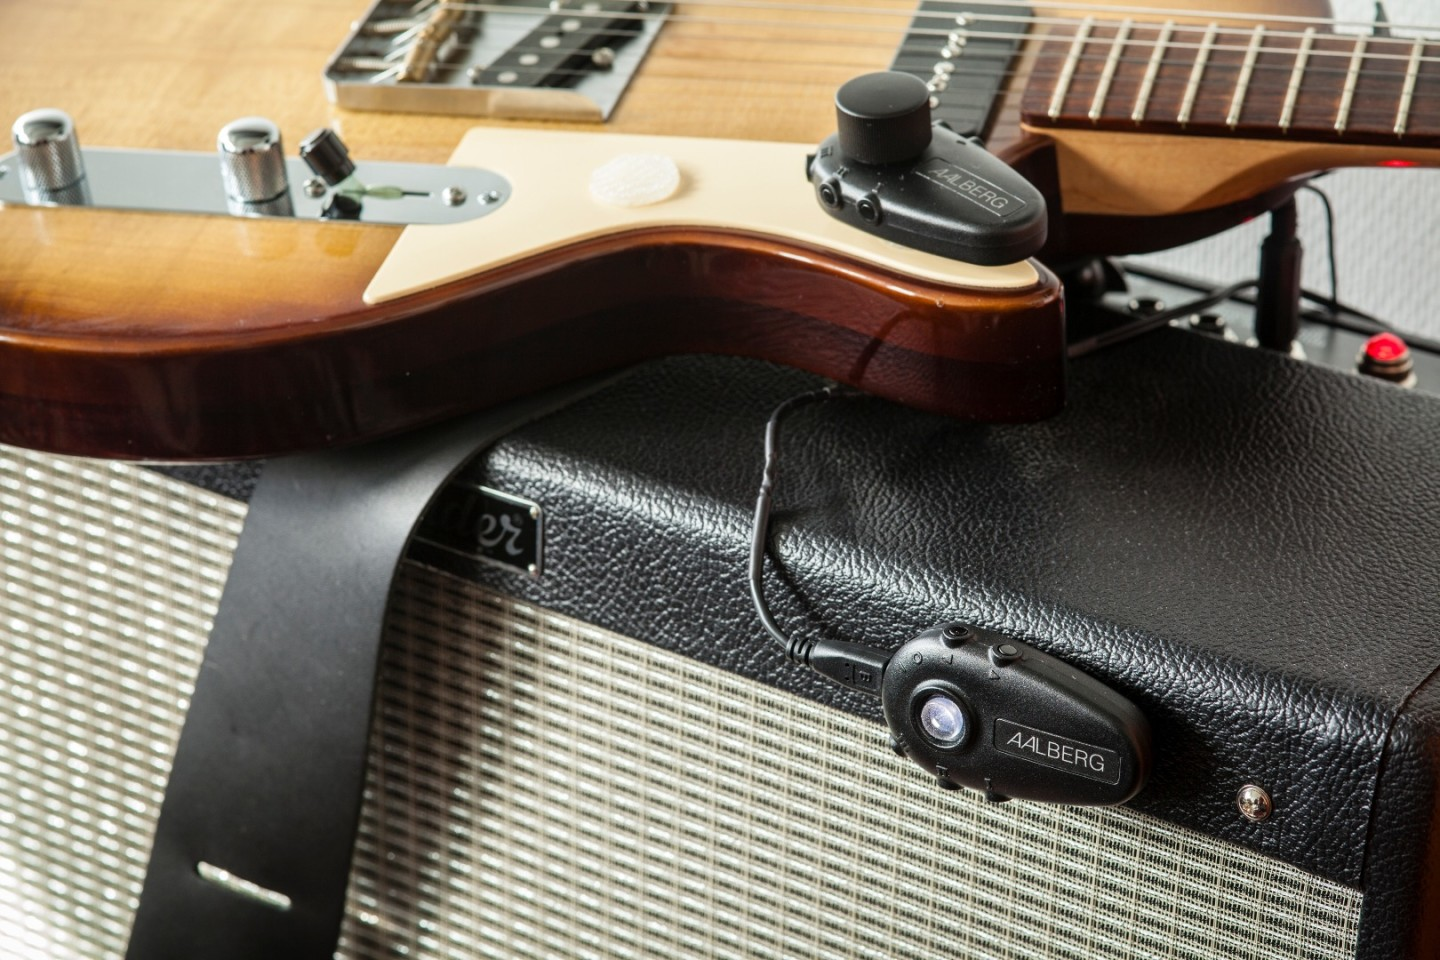
\includegraphics[width=\textwidth]{moon1}

Głównym plusem urządzenia jest to, że ma dedykowany odbiornik.
Minusy:

\begin{itemize}
\item Ma tylko jeden duży przycisk, reszta jest w takim miejscu, do którego jest trudno się dostać palcami, szczególnie podczas aktywnego grania
\item Projekt na kickstarterze został zawieszony, więc nie ma oficjalnej możliwości zakupu
\end{itemize}

\pagebreak
\section{Wyzwania}

Poniżej są wymienione problemy, których rozwiązanie jest niezbędne do realizacji projektu:
	
\begin{itemize}
\item Wybór urządzeń i protokołu do bezprzewodowej transmisji danych
\item Wybór mikrokontrolerów do zaimplementowania całej logiki
\item Zapewnienie minimalnego możliwego poboru mocy
\item Zapewnienie minimalnego możliwego czasu reakcji
\item Wybór stacku technologicznego z należnym wsparciem
\item Dostosowanie się do ograniczeń sprzętowych mikrokontrolerów
\item Rozwiązanie problemu parowania urządzeń bezprzewodowych
\item Dostosowanie się do wymagań interfejsu MIDI
\item Stworzenie lightweight interfejsu do konfigurowania systemu
\item Integracja z urządzeniami zewnętrznymi (wzmacniacz, karta muzyczna itp)
\end{itemize}

\section{Struktura pracy}
W drugiej części pracy jest opisany zakres projektu oraz wybrane rozwiązania technologiczne.

W trzeciej części opisany jest standard MIDI, komunikacja przez BLE oraz API do konfigurowania urządzenia.

W czwartej części przejdziemy do szczegółowego opisu implementacji ze schematami, kodem źródłowym, konfiguracją modułów BLE, sposobami zaprogramowania mikrokontrolerów, opisem API oraz informacjami na temat napisania GUI.

\pagebreak
\chapter{Cel i zakres}
Celem projektu jest zbudowanie prototypu, który jest w stanie zademonstrować całą drogę od wciśnięcia przycisku na nadajniku do zmiany ustawienia na wzmacniaczu.
Projekt nie obejmuje stworzenia płytki drukowanej oraz obudowy.

\section {Zakres}
Komponenty systemu:

\begin{itemize}
\item Nadajnik
	
\begin{itemize}
\item Zasilany małą baterią CR2025
\item Reaguje na wciśnięcia przycisków
\item Wysyła informację o wciśnięciu przycisku do odbiornika bezprzewodowo
\end{itemize}

\item Odbiornik
	
\begin{itemize}
\item Nasłuchuje komunikaty nadajnika
\item Ma strukturę danych która mapuje numery przycisków na konkretny komunikat MIDI (może to być sekwencja komunikatów, z której jest wybierany kolejny komunikat po każdym wciśnięciu przycisku)
\item Udostępnia interfejs do konfigurowania mapowania opisanego wyżej
\item Wysyła komunikat MIDI na interfejs DIN-5
\end{itemize}

\item Aplikacja do konfigurowania odbiornika
	
\begin{itemize}
\item Używa interfejsu udostępnionego przez odbiornik
\item Zapewnia łatwy user-friendly sposób na konfigurowanie odbiornika
\end{itemize}

\end{itemize}

\pagebreak
\section {Stack technologiczny}

\subsection{Sprzęt}
\paragraph{HM-10}\mbox{} \\
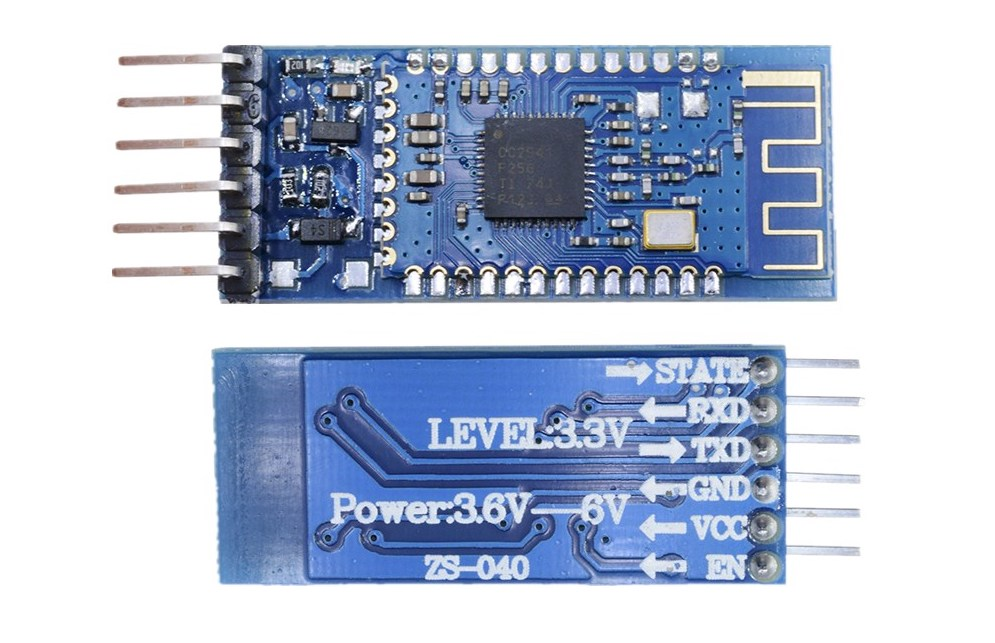
\includegraphics[width=\textwidth]{hm-10}

Do komunikacji bezprzewodowej został wybrany moduł BLE HM-10. Jest następcą dobrze znanego HC-05. Specyfika projektu wymaga urządzenia bezprzewodowego, które nie tylko ma mały pobór mocy, a również szybki czas reakcji. Z jednej strony mamy WiFi, które zapewnia niski czas reakcji, ale pobiera dużo prądu. Z innej strony mamy urządzenia IoT, które potrafią prawie nie zużywać prądu, ale przebywają w trybie deep sleep, wyjście z którego niestety potrzebuję czasu, na który nie możemy sobie pozwolić w przypadku tego projektu. Kompromisem jest bluetooth, a konkretnie BLE. Jest idealnym kompromisem pomiędzy poborem mocy i czasem reakcji.

Wybór był spowodowany następującymi cechami modułu:
\begin{itemize}
\item Najpopularniejszy jeśli chodzi o moduły BLE, więc ma dobre wsparcie
\item Prosty interfejs (zasilanie, masa, piny TX/RX do transmisji)
\item Obsługuje komendy AT
\item Przystępna cena (około 20 zł)
\end{itemize}

\pagebreak
\paragraph{Attiny85}\mbox{} \\
\begin{center}
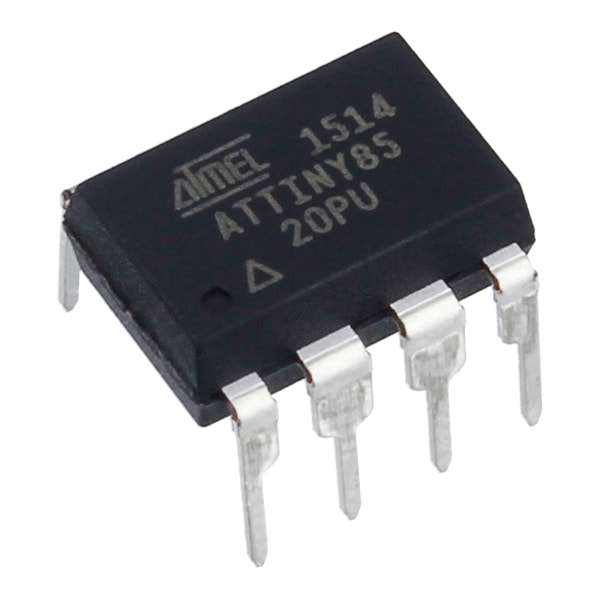
\includegraphics[width=6cm]{attiny}
\linebreak
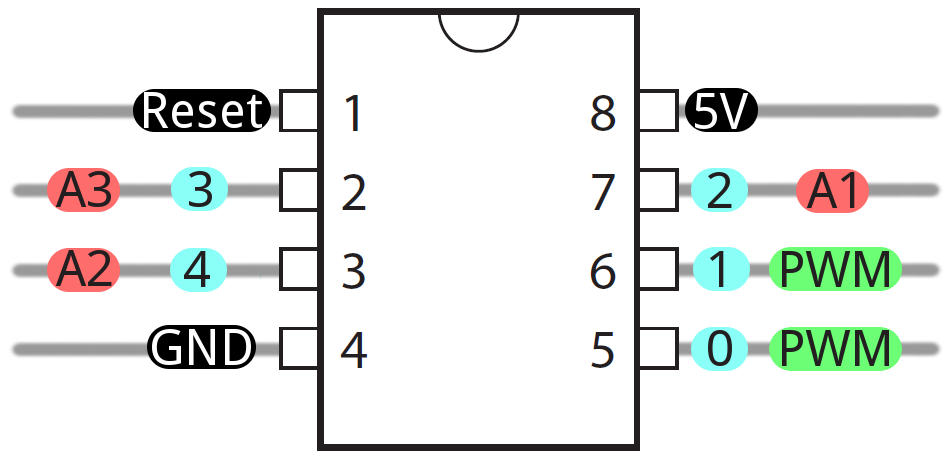
\includegraphics[width=9cm]{attiny-pinout}
\end{center}

Do komunikacji z modułem BLE potrzebujemy mikrokontrolera. Wybór padł na ATtiny85 z następujących powodów:

\begin{itemize}
\item Wspiera język Arduino, więc jest łatwy w zaprogramowaniu
\item Ma bardzo dobre wsparcie, więc łatwo jest znaleźć informację i się nauczyć na przykładzie innych projektów
\item Pobiera bardzo mało prądu (około 4 razy mniej niż moduł BLE)
\item Jest bardzo kompaktowy (rozmiarem z przycisk)
\item Ma 2 piny do zasilania oraz 6 pinów I/O, czego wystarczy do komunikacji z modułem BLE oraz podpięcia czterech przycisków
\item Przystępna cena (około 10 zł)
\end{itemize}

\paragraph{ESP-32}\mbox{} \\
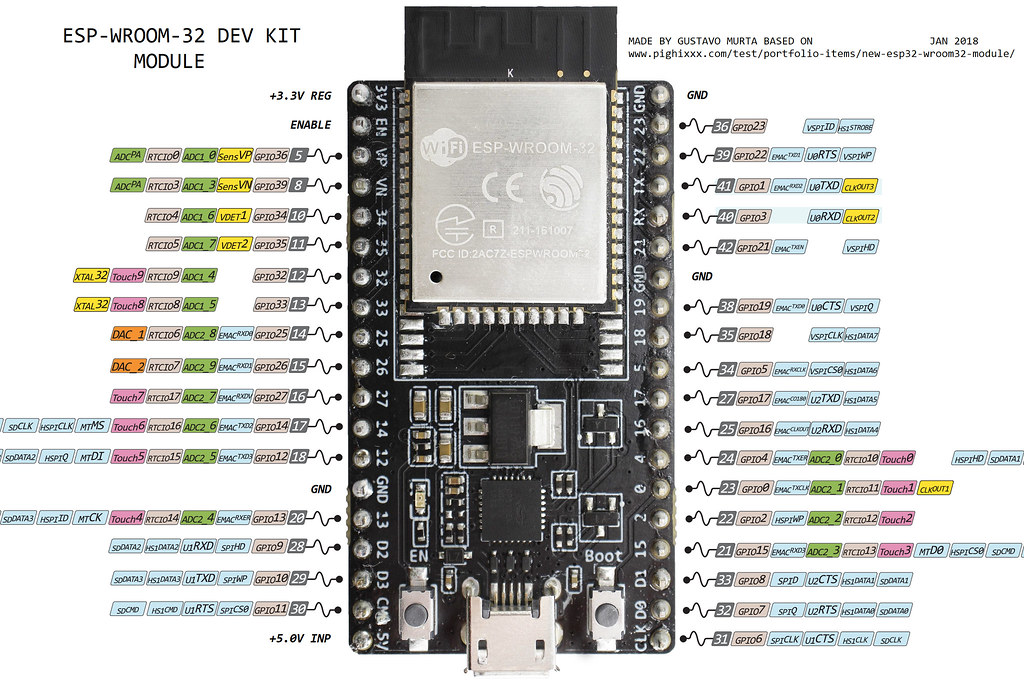
\includegraphics[width=\textwidth]{esp-32-pinout}
W przypadku odbiornika musimy zapewnić:
\begin{itemize}
\item Przechowywanie struktury danych z mapowaniem
\item Komunikację z modułem BLE
\item Komunikację z interfejsem MIDI
\item Interfejs do konfigurowania
\end{itemize}

Jest dużo więcej funkcjonalności, natomiast nie ma ograniczenia na pobór mocy. Rozważana była możliwość użycia tego samego modułu BLE do interfejsu konfigurowania, natomiast to uniemożliwia jednoczesną konfigurację i testowanie przesyłu danych, ponieważ urządzenie BLE w trybie slave może trzymać tylko jedno połączenie. Prostszym rozwiązaniem jest użycie WiFi i stworzenie web serwera z REST API do konfigurowania mapowania.

Wybrany został moduł ESP-32:

\begin{itemize}
\item Wspiera język MicroPython, jest łatwiejszy niż mieszanka Arduino i C++, ma frameworki webowe
\item Ma bardzo dobre wsparcie, jest kontynuacją ESP8266 i ma wielkie community
\item Ma zintegrowane WiFi, może działać jak w trybie stacji, tak i punktu dostępu
\item Przystępna cena (około 30 zł, zależy od konkretnej płyty)
\end{itemize}

\subsection{Oprogramowanie}
\paragraph{Nadajnik}\mbox{} \\

Mikrokontroler Attiny85 jest zaprogramowany w języku Arduino z użyciem rozszerzenia w C++ do debounce-owania przycisków. Jest to niezbędne, żeby wciśnięcie przycisku nie powodowało zakłóceń w postaci wykrycia dodatkowych wciśnięć.
Została użyta biblioteka \texttt{SofwareSerial} do komunikacji z modułem BLE przez piny TX/RX.
\paragraph{Odbiornik}\mbox{} \\

Odbiornik został zaprogramowany całkowicie w języku MicroPython. Do WiFi została użyta wbudowana biblioteka \texttt{network}. Do komunikacji z modułem BLE oraz interfejsem MIDI - biblioteka \texttt{machine.UART}.
Do implementacji REST API do wyboru są frameworki
\begin{itemize}
\item Picoweb
\item MicroWebSrv
\item MicroWebSrv2
\end{itemize}

Podczas researchu frameworku Picoweb zauważyłem problemy z zależnościami, co było znakiem słabego wsparcia. MicroWebSrv2 jest ulepszoną wersją MicroWebSrv, natomiast kiedy testowałem tą wersję frameworku - zapytania się wykonywały kilka razy dłużej.

Wybrany został MicroWebSrv dlatego, że zadowala potrzebę, i mimo, że kod nie jest najlepszej jakości (nie stosuje zasad PEP8), jest tego kodu bardzo mało (880 linijek). Co sprawia, że w przypadku braku wsparcia, naprawa problemów z frameworkiem samodzielnie jest też możliwa.
\paragraph{Konfigurator}\mbox{} \\

Aplikacja desktopowa została napisana w języku Python w frameworku Kivy. Ten framework został wybrany, ponieważ:
\begin{itemize}
\item Ma bardzo dobrą dokumentację
\item Out-of-the-box zapewnia responsywny layout (czego nie ma na przykład w najpopularniejszym frameworku Tkinter)
\item Domyślne widgety (przyciski, napisy) już wyglądają dobrze i nie wymagają customizacji stylistycznej
\end{itemize}

\pagebreak
\chapter{Projekt systemu}
\section{Standard MIDI}

MIDI (Musical Instrument Digital Interface) - jest to standard definiujący interfejs komunikacyjny pomiędzy urządzeniami muzycznymi (komputery, karty dźwiękowe, syntezatory, wzmacniacze itp). Został stworzony w 1983 roku.
Poniżej jest przedstawiona struktura przykładowego komunikatu MIDI.
\linebreak

\subsection{Komunikaty MIDI}
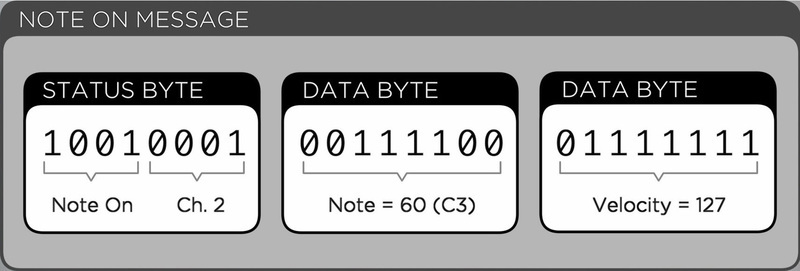
\includegraphics[width=\textwidth]{midi-message}

Komunikat MIDI składa się z trzech bajtów, pierwszy bajt jest bajtem statusu (określa typ wiadomości oraz kanał), kolejne dwa są bajtami danych i mają różne znaczenia w zależności od typu komunikatu.
Drzewo poniżej przedstawia wszystkie możliwe typy komunikatów MIDI. W tym projekcie skupiamy się na komunikatach głosowych.

\Tree[.\text{Komunikaty MIDI} [.Kanałowe [.\textbf{Głosowe} ] [.\text{Trybu pracy} ] ] [.Systemowe [.Wspólne ] [.\text{Czasu rzeczywistego} ] [Niestandardowe ] ] ]

\paragraph{Komunikaty głosowe}\mbox{} \\

\begin{table}[]
\begin{tabular}{|l|l|l|l|l|}
\hline
\textbf{Typ komunikatu}    &  \textbf{Bajt statusu} & \textbf{Bajt danych 1} & \textbf{Bajt danych 2}  \\ \hline
Note off                   &  8x                    &    Key number          &  Note Off velocity  	   \\ \hline
Note on                    &  9x                    &    Key number          &  Note on velocity       \\ \hline
Polyphonic Key Pressure    &  Ax                    &    Key number          &  Amount of pressure     \\ \hline
Control Change             &  Bx                    &    Controller number   &  Controller value       \\ \hline
Program Change             &  Cx                    &    Program number      &  None                   \\ \hline
Channel Pressure           &  Dx                    &    Pressure value      &  None                   \\ \hline
Pitch Bend                 &  Ex                    &    MSB                 &  LSB                    \\ \hline
\end{tabular}
\end{table}

Do testowania najwygodniej jest wykorzystać komunikaty \textit{Note On} oraz \textit{Note Off} ponieważ jest łatwo monitorować te komunikaty na ścieżkach w programach muzycznych (DAW).

\subsection{Złącze MIDI}
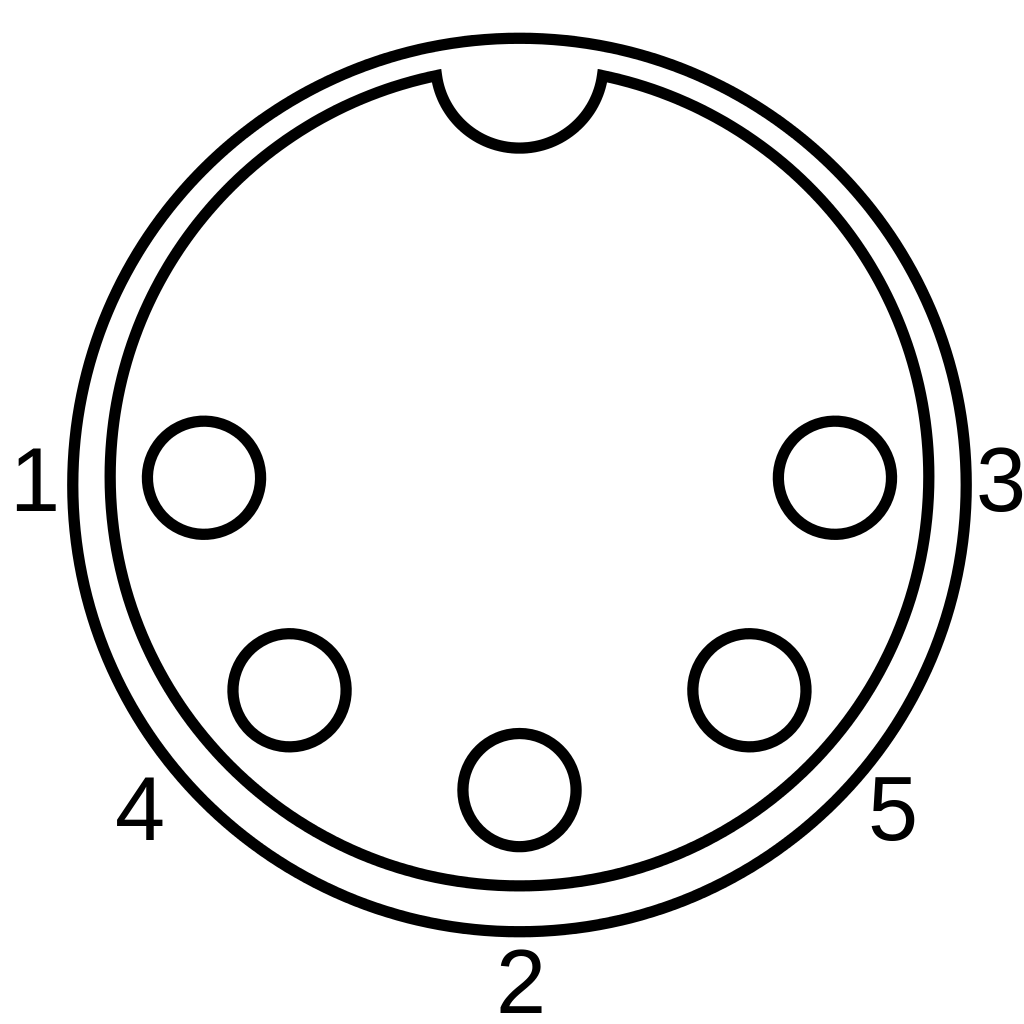
\includegraphics[width=6cm]{midi-jack}

Złącze MIDI posiada 5 pinów. Może działać jak na 3.3V tak i na 5V.
Dane są przesyłane szeregowo z baud rate-m 31,250.

\begin{enumerate}
\item Nieużywany
\item GND
\item Nieużywany
\item Dane
\item VCC
\end{enumerate}

\newpage
\section{Obsługa modułów BLE}

Moduły BLE są konfigurowane za pomocą komend AT (albo inaczej "\textit{Hayes command set}"). Zbiór tych komend jest trochę specyficzny, ponieważ projekcie został użyty klon klona oryginalnego modułu HM-10 \textbf{MLT-BT05}.
Całą listę komend można znaleźć \href{http://denethor.wlu.ca/arduino/MLT-BT05-AT-commands-TRANSLATED.pdf}{tutaj}.

Interesują nas natomiast:

\begin{table}[htb]
\begin{tabular}{|l|l|p{6cm}|}
\hline
\textbf{Opis}    &  \textbf{Komenda} & \textbf{Parametr}  \\ \hline
Ustawienie trybu                   &  AT+ROLE<Param>          &  0 - slave, 1 - master  	   \\ \hline
Sprawdzenie wersji                    &  AT+VERSION           &  N/A       \\ \hline
Ustawienie nazwy    &  AT+NAME<Param>              &  <nazwa>     \\ \hline
Restart modułu             &  AT+RESET            & N/A      \\ \hline
Wyszukiwanie modułów             &  AT+INQ<Param>        &  1 - zacząć skan, 0 - skończyć skan                   \\ \hline
Nawiązanie połączenia           &  AT+CONN<Param>                    &  0-7                   \\ \hline
Tryb startowy                 &  AT+IMME<Param>                    &  0 - start w trybie komend, 1 - start w trybie normalnym                    \\ \hline
Włączenie trybu transmisji                 &  AT+START                    &  N/A                    \\ \hline
Ustawienia notyfikacji                 &  AT+NOTI<Param>                    &  1 - wysyłaj notyfikacje, 0 - nie wysyłaj                    \\ \hline
Reset do ustawień fabrycznych                 &  AT+DEFAULT                    &  N/A                    \\ \hline
\end{tabular}
\end{table}

\section{REST API}

Struktura danych do przechowywania mapowań przycisków do sekwencji komunikatów wygląda następująco:

\lstset{
    string=[s]{"}{"},
    stringstyle=\color{blue},
    comment=[l]{:},
    commentstyle=\color{black},
}
\begin{lstlisting}
{
  "notes": [
    [
      [
        200,
        100,
        100
      ],
      [
        128,
        123,
        150
      ]
    ],
    [[234, 234, 234]],
    []
  ]
}
\end{lstlisting}

Na serwerze jest wystawiony jeden endpoint wspierający zapytania GET do pobrania konfiguracji oraz POST do nadpisywania.

\chapter{Implementacja}
\section{Nadajnik}
\subsection{Schemat do zaprogramowania ATTINY85}

Przedstawiony poniżej schemat pokazuje jak za pomocą Arduino Nano zaprogramować chip ATTINY85.

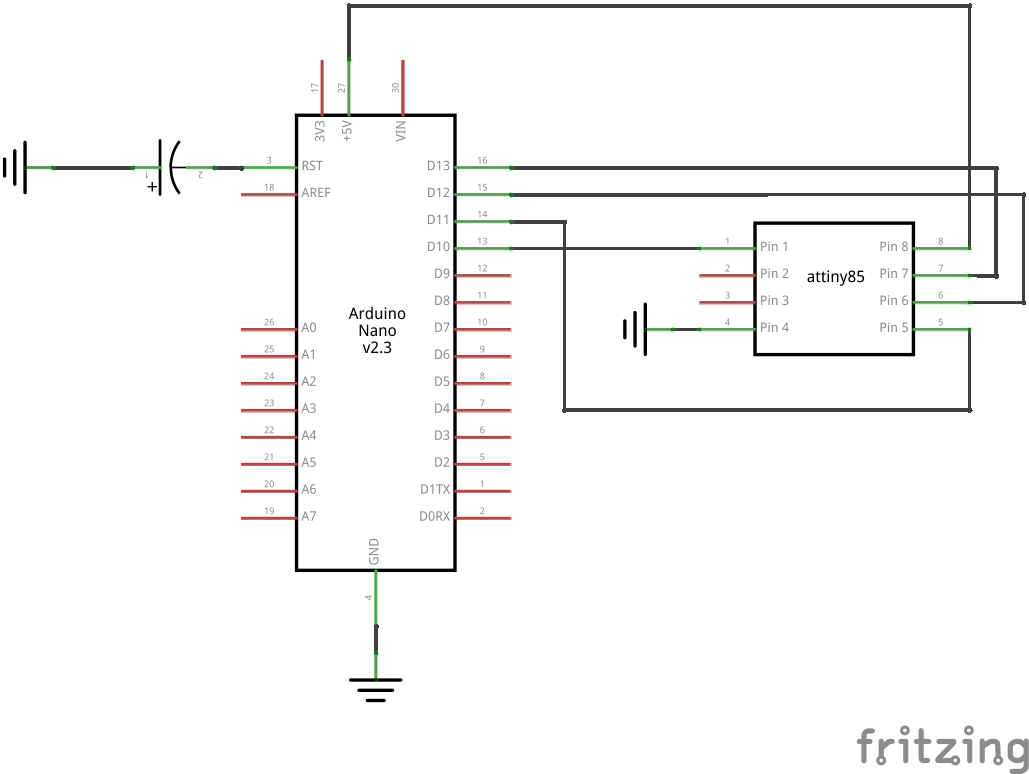
\includegraphics[width=\textwidth]{attiny-prog-schem}
\newpage
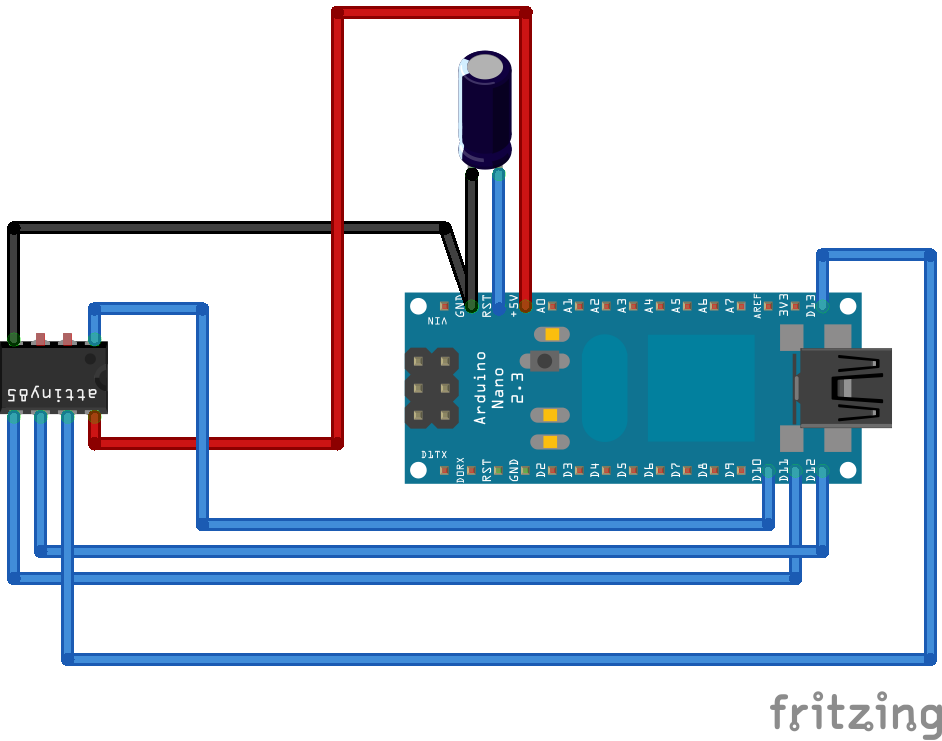
\includegraphics[width=\textwidth]{attiny-prog-bb}

Do zaprogramowania ATTINY również niezbędne są odpowiednie ustawienia w Arduino IDE.
Należy pobrać definicje mikrokontrolerów serii ATTINY, wybrać odpowiedni model (w naszym przypadku ATTINY85), ustawić zegar na 8 MHz.

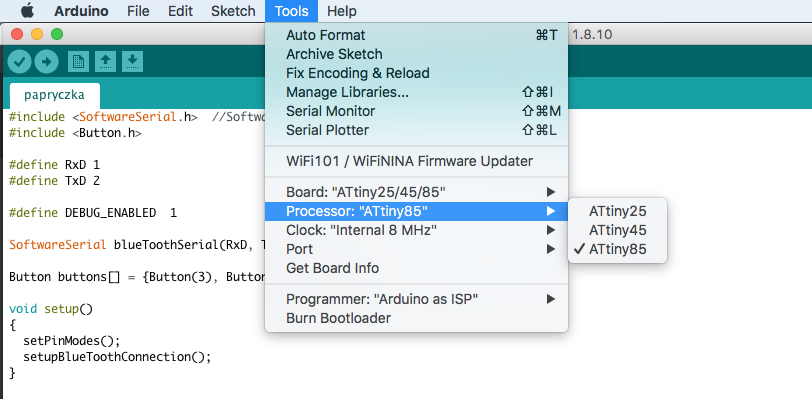
\includegraphics[width=\textwidth]{arduino-settings}

\pagebreak
\subsection{Schemat standalone}

Przedstawiony poniżej schemat pokazuje jak połączyć zaprogramowany chip ATTINY z modułem BLE i trzema przyciskami.
Warto również zauważyć, że system jest bardziej stabilny (rzadziej traci połączenie) jeśli użyjemy dwóch baterii CR2032 podłączonych równolegle.

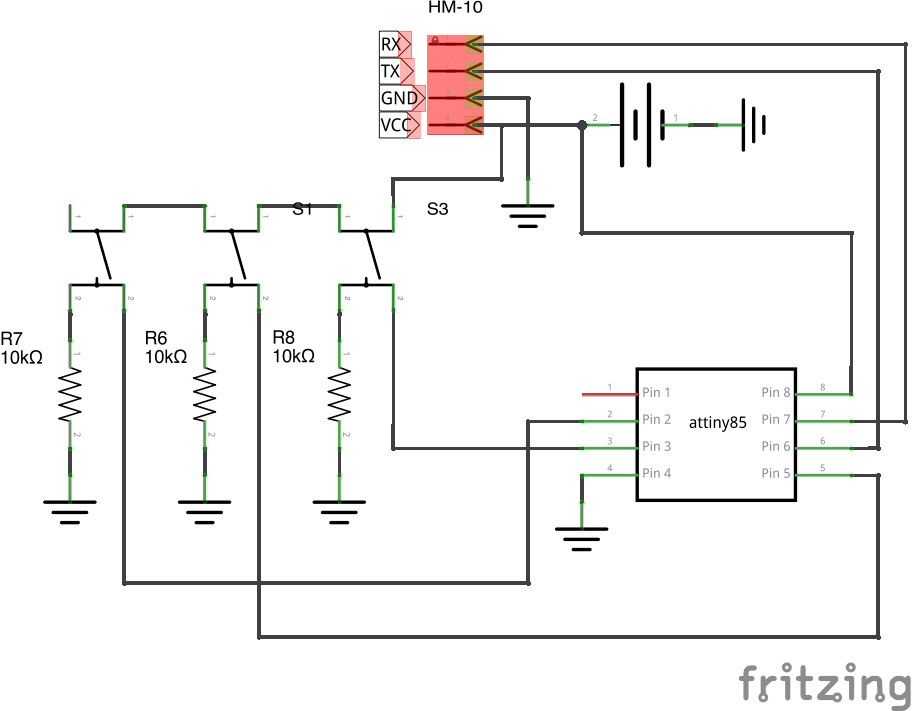
\includegraphics[width=\textwidth]{nadajnik-schem}
\newpage
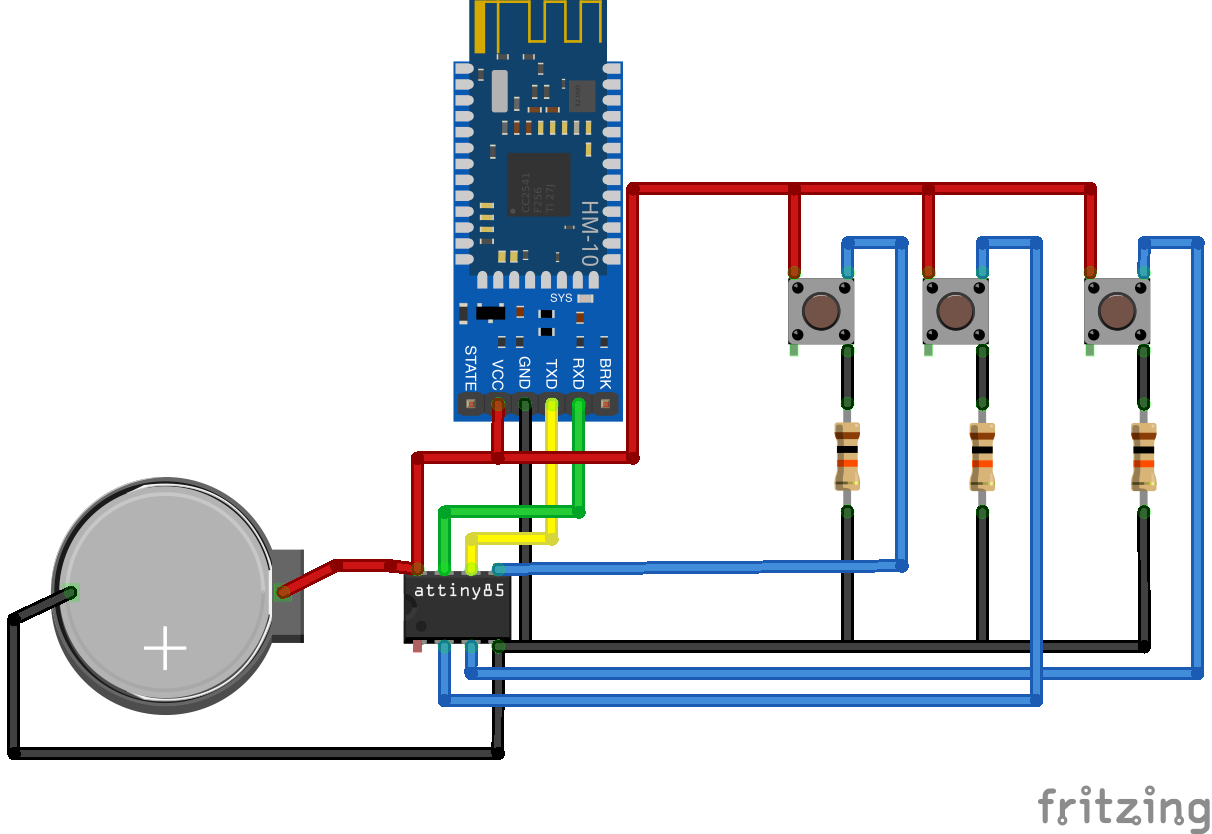
\includegraphics[width=\textwidth]{nadajnik-bb}
\subsection{Ustawienie modułu BLE jako slave}

Przedstawiona poniżej funkcja jest użyta do konfigurowania modułu BLE na nadajniku jako slave.
Moduł jest resetowany do ustawień fabrycznych, dostaje przypisaną nazwę, ustawia się w tryb slave z startowaniem w trybie komend z włączonymi notyfikacjami.

\begin{lstlisting}[language=Arduino]
void setupBlueToothConnection()
{
  blueToothSerial.begin(9600);
  write("DEFAULT");
  write("RESET");
  write("NAMEpapryczka");
  write("ROLE0");
  write("IMME0");
  write("RESET");
  write("NOTI1");
  blueToothSerial.flush();
}
\end{lstlisting}

\pagebreak
\subsection{Obsługa przycisków}

Z wysokiego poziomu obsługa przycisków wygląda następująco. Definiujemy trzy przyciski wskazując piny I/O na ATTINY85.
Później w nieskończonej pętli programu cały czas sprawdzamy stan przycisków. Jeśli jest wciśnięty - wysyłamy przez bluetooth numer przycisku.

\begin{lstlisting}[language=Arduino]
Button buttons[] = {Button(3), Button(0), Button(4)};

...

void loop() {
  for (int i = 0; i < 3; i++) {
    checkButton(&buttons[i], i);
  }
}

void checkButton(Button* button, int message) {
    if(button->check(blueToothSerial)) { 
        blueToothSerial.print(message);
    }
}
\end{lstlisting}

Typowym problemem z implementacją przycisków jest tak zwany \textit{"debounce"}. Chodzi o to, że podczas wciśnięcia przycisku jest generowany szum w postaci szybko zmieniających się wartości logicznych. Logika, która rozwiązuje ten problem została wyniesiona do biblioteki \textit{Button.h}.
Przed kompilacją programu należy upewnić się, że w ustawieniach Arduino IDE jest podana właściwa ścieżka do bibliotek zewnętrznych.

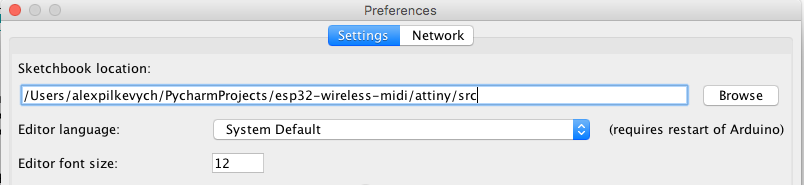
\includegraphics[width=\textwidth]{arduino-libraries}

Problem został rozwiązany w następujący sposób. Jeśli przycisk ma stan logiczny 1 - sprawdzamy czy od ostatniego wciśnięcia minęło 10 milisekund. Jeśli tak - raportujemy wciśnięcie, jeśli nie - traktujemy to jako szum i ustawiamy aktualny czas jako czas ostatniego wciśnięcia.

\pagebreak

\begin{lstlisting}[language=C++]
Button::Button(int pin)
{
  pinMode(pin, INPUT);
  this->_pin = pin;
}

bool Button::check(SoftwareSerial bt)
{
  int reading = digitalRead(this->_pin);

  if (reading == this->lastButtonState) {
    return false;
  }

  bool isNoise = ((millis() - this->lastPress) < this->debounceDelay);

  this->lastPress = millis();
  this->lastButtonState = reading;

  bool buttonPressed = !isNoise && reading == HIGH;

  return buttonPressed;
}
\end{lstlisting}

\pagebreak

\section{Odbiornik}
\subsection{Schemat}

Przedstawiony poniżej schemat pokazuje jak podłączyć do modułu ESP-32 moduł BLE, złącze MIDI oraz diodę sygnalizującą odebranie komunikatu z nadajnika.

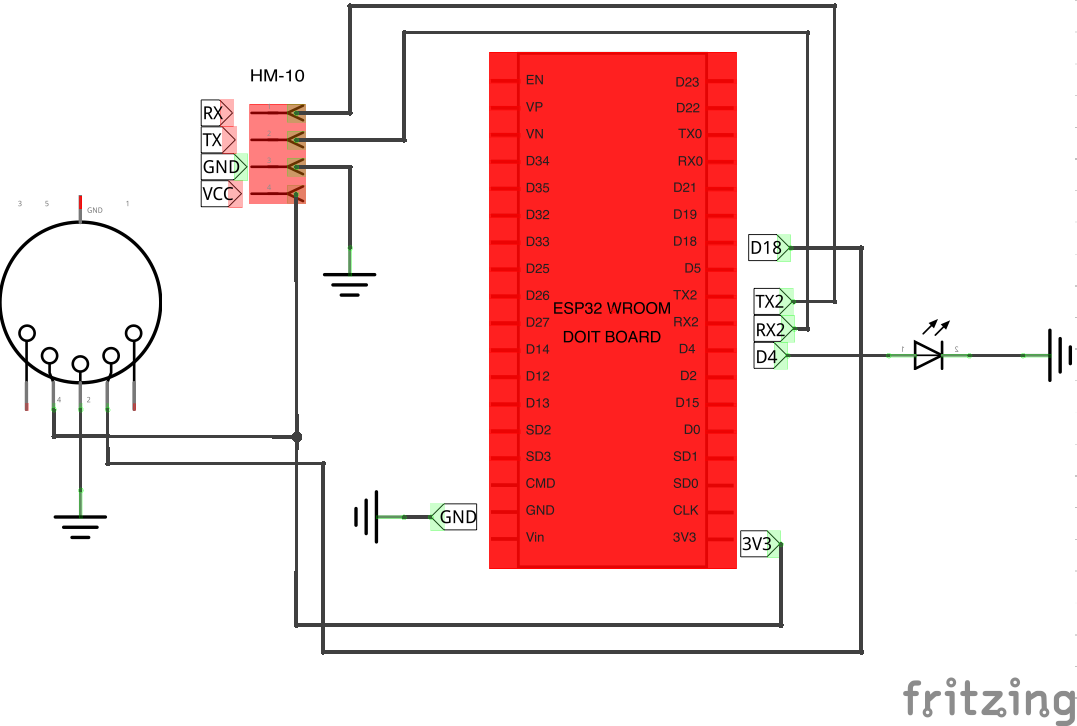
\includegraphics[width=\textwidth]{odbiornik-schem}
\newpage
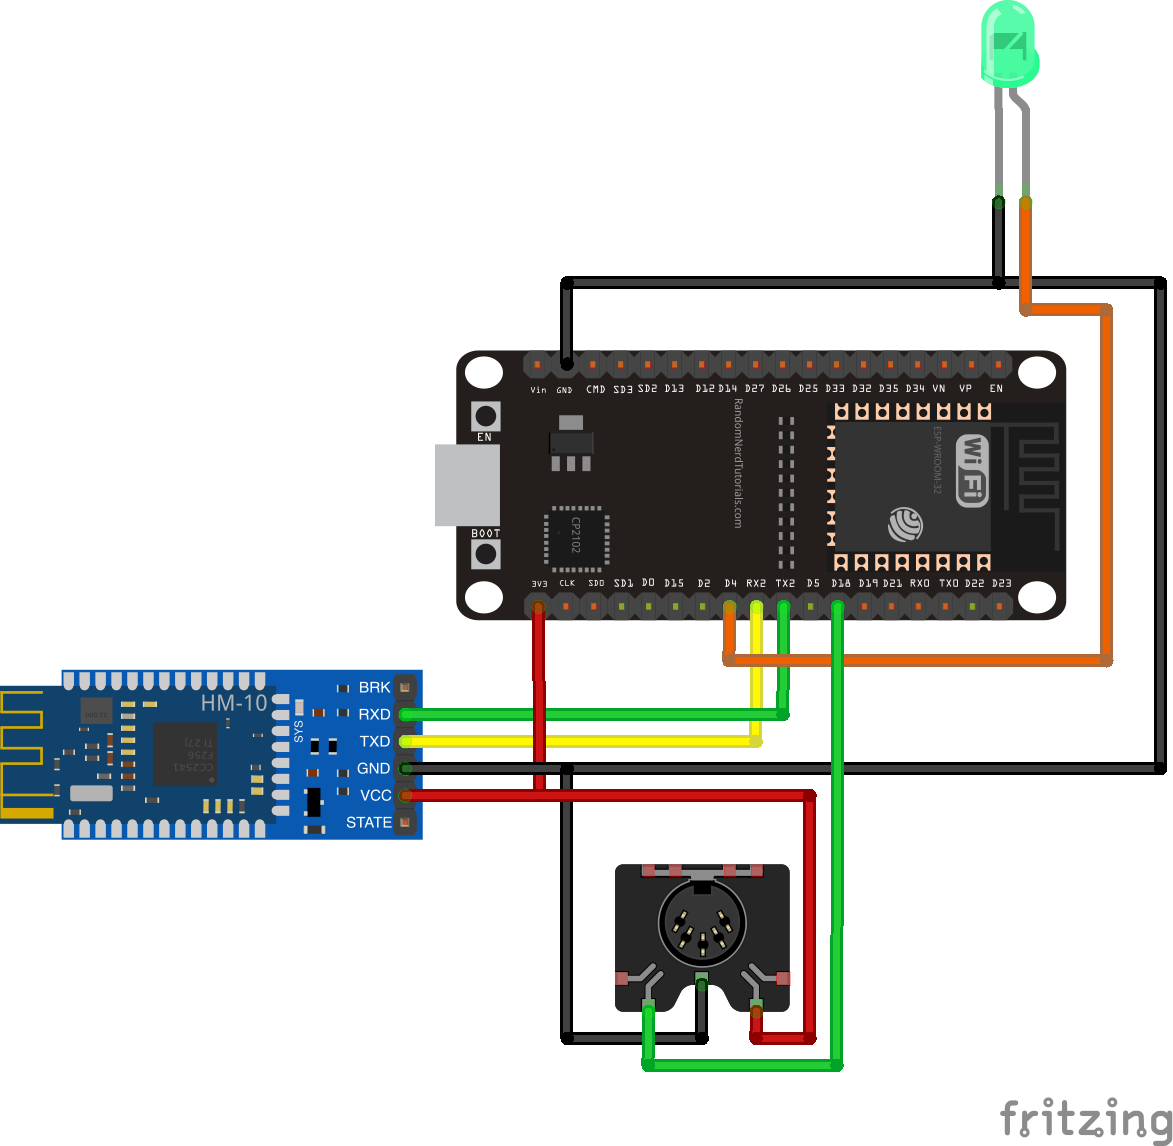
\includegraphics[width=\textwidth]{odbiornik-bb}
\newpage
\subsection{Zaprogramowanie}

Żeby zaprogramować moduł ESP-32 w języku Python - należy wgrać na płytkę interpreter. Po czym można się podłączyć do konsoli Python-owej przez (na przykład) wtyczkę MicroPython dla PyCharm IDE.

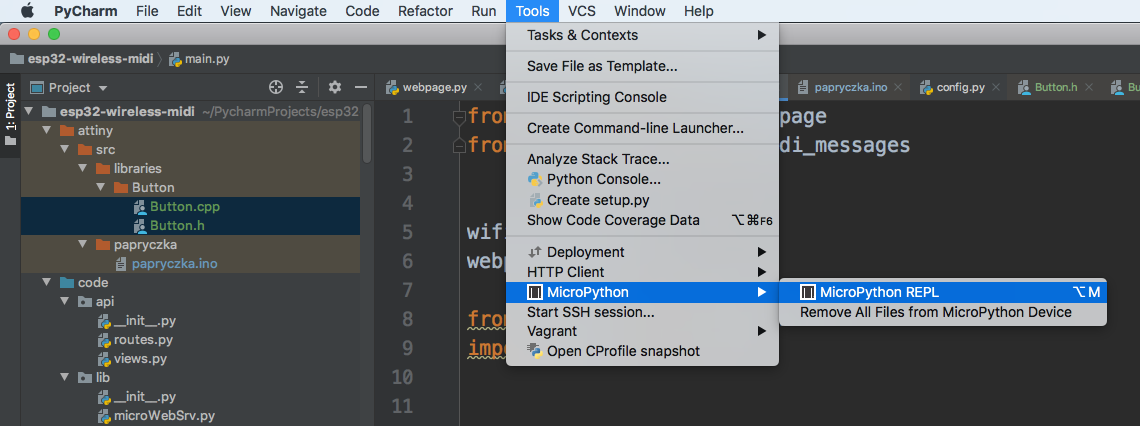
\includegraphics[width=\textwidth]{pycharm}

Przykładowe logi aplikacji odbiornika wyglądają tak:

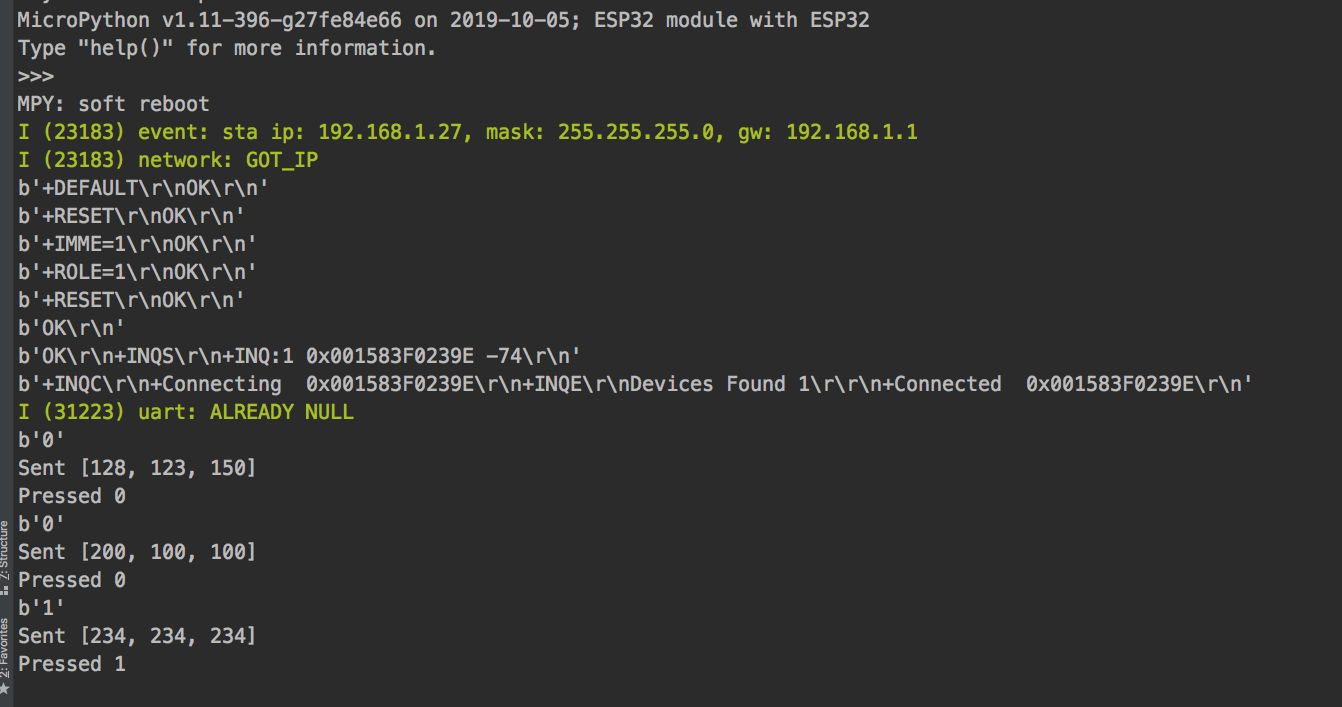
\includegraphics[width=\textwidth]{logs}

Należy uważać, ponieważ płytka potrafi obsłużyć tylko jedno połączenie. Jeśli nie wyłączymy terminal to nie będzie można wgrać plik.

Podczas startu iterpreter Pythona automatycznie odpala plik \textit{main.py}. Ten plik jest punktem wejściowym do aplikacji.

Zarządzać plikami można (na przykład) przez narzędzie konsolowe \textit{ampy}. Pozwala ono na wgrywanie, pobieranie oraz usuwanie plików/katalogów z płytki.

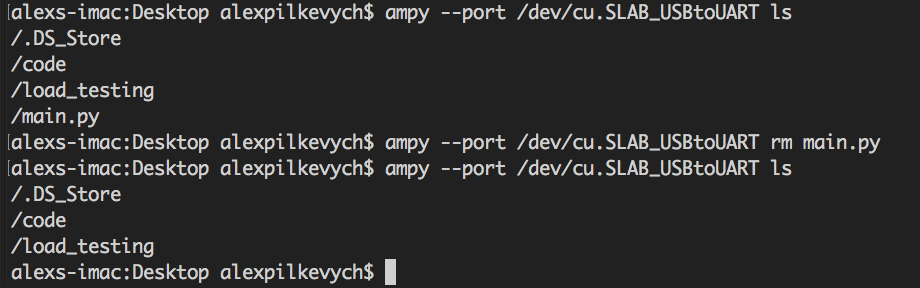
\includegraphics[width=\textwidth]{ampy}


\subsection{Konfiguracja WiFi}

ESP-32 wspiera jak tryb Access Point (punkt dostępu) tak i Station (tryb stacji). W środowisku testowym podłączenie płytki jako stacji do sieci domowej pozwala na korzystanie z internetu w trakcie testowania aplikacji. W środowisku docelowym musimy jednak zapewnić tryb punktu dostępu, ponieważ urządzenie powinno być przenośne i niezależne od innych sieci. Z tych powodów obydwa tryby zostały zaimplementowane. Da się je przełączyć odpowiednio ustawiając zmienną \textit{ACCESS\_POINT\_MODE}. W obu przypadkach używamy tego samego adresu IP, ponieważ jest zahardkodowany w aplikacji konfigurującej odbiornik.


\begin{lstlisting}[language=Python]
ACCESS_POINT_MODE = True


class AccessPointConfig:
    SSID = 'ESP-32-WOOWOOWOO'
    PASSWORD = 'thisisnotaspoon'
    IP = '192.168.1.27'
    SUBNET_MASK = '255.255.255.0'
    GATEWAY = '192.168.1.27'


class StationConfig:
    SSID = '<SSID>'
    PASSWORD = '<PASSWORD>'
    IP = '192.168.1.27'
    SUBNET_MASK = '255.255.255.0'
    GATEWAY = '192.168.1.1'
\end{lstlisting}

\pagebreak

\begin{lstlisting}[language=Python]
import network
from code import config


def connect_station(c: config.StationConfig):
    station = network.WLAN(network.STA_IF)
    station.active(True)
    station.connect(c.SSID, c.PASSWORD)
    station.ifconfig((c.IP, c.SUBNET_MASK, c.GATEWAY, '8.8.8.8'))


def connect_access_point(c: config.AccessPointConfig):
    ap = network.WLAN(network.AP_IF)
    ap.active(True)
    ap.config(essid=c.SSID, password=c.PASSWORD)
    ap.ifconfig((c.IP, c.SUBNET_MASK, c.GATEWAY, '8.8.8.8'))


def start_wifi():
    if config.ACCESS_POINT_MODE:
        connect_access_point(config.AccessPointConfig())
    else:
        connect_station(config.StationConfig())

\end{lstlisting}

\pagebreak
\subsection{Ustawienie modułu BLE jako master}

Poniżej jest przedstawiona klasa, odpowiedzialna za ustawienie modułu BLE w trybie master i nasłuchiwanie.

\begin{lstlisting}[language=Python]
class Receiver:

    def connect(self):
        self.factory_default()
        self.reset()
        self.set_imme()
        self.set_master()
        self.reset()
        self.start()
        self.inquire()
        self.connect_first()
        ...

    def run_command(self, command):
        self.uart.write(command+'\r\n')
        time.sleep(1)
        return self.wait()

    def reset(self):
        return self.run_command('AT+RESET')

    def factory_default(self):
        return self.run_command('AT+DEFAULT')

    def set_master(self):
        return self.run_command('AT+ROLE1')

    def set_imme(self):
        return self.run_command('AT+IMME1')

    def start(self):
        return self.run_command('AT+START')

    def inquire(self):
        return self.run_command('AT+INQ')

    def connect_first(self):
        return self.run_command('AT+CONN1')

    def wait(self):
        data = None
        while not data:
            data = self.read()
        print(data)
        return data
\end{lstlisting}

Żeby tą klasę użyć wystarczy odpalić:

\begin{lstlisting}[language=Python]
Receiver().connect()
\end{lstlisting}

Wtedy są wykonywane następujące działania:

\begin{enumerate}
\item Utworzenie połączenia szeregowego z modułem BLE	
\item Reset do ustawień fabrycznych
\item Restart modułu
\item Ustawienie trybu komend
\item Ustawienie trybu master
\item Restart modułu
\item Włączenie trybu transmisji
\item Skanowanie urządzeń
\item Nawiązanie połączenia
\end{enumerate}

W tym momencie mamy sparowane moduły BLE, można zauważyć, że czerwona dioda na modułach przestaje mrugać i stabilnie się świeci.

\newpage
\subsection{Nasłuchiwanie}

W momencie kiedy połączenie pomiędzy modułami BLE na nadajniku i odbiorniku zostało nawiązane, wykonywane są następujące czynności:

\begin{enumerate}
\item Utworzenie połączenia szeregowego z interfejsem MIDI
\item Początek nasłuchiwania w pętli nieskończonej.
\begin{itemize}
\item W przypadku komunikatu \textit{Disconnected} wywołujemy próbę nawiązania nowego połączenia w nowej pętli nieskończonej
\item W przypadku liczby od 0-2 jest triggerowane wysyłanie następnego w sekwencji komunikatu MIDI dla danego przycisku
\end{itemize}
\end{enumerate}


\begin{lstlisting}[language=Python]
class MidiInterface:
    baud = 31250

    def __init__(self):
        self.uart = None

    def connect(self):
        self.uart = UART(2, self.baud)
        self.uart.init(self.baud, bits=8, parity=None, stop=1, tx=18)

    def send(self, slot):
        if midi_messages.slots.messages[slot]:
            message = midi_messages.slots.pop_message(slot)
            self.uart.write(bytes(message))
            print('Sent {}'.format(message))
\end{lstlisting}

\newpage
\begin{lstlisting}[language=Python]
class Receiver:
    def __init__(self):
    	...

        self.EVENTS = {
            b'Disconnected': self.reconnect,
            b'0': lambda: self.on_button(0),
            b'1': lambda: self.on_button(1),
            b'2': lambda: self.on_button(2)
        }
        self.midi = MidiInterface()

    def connect(self):
        ...
        self.midi.connect()
        self.loop()

    def on_button(self, slot):
        self.led.on()
        self.midi.send(slot)
        self.led.off()
        print('Pressed {}'.format(slot))

    def reconnect(self):
        while True:
            data = self.connect_first()
            if b'Connected' in data:
                return self.loop()
            time.sleep(1)

    def read(self):
        return self.uart.read()

    def wait(self):
        data = None
        while not data:
            data = self.read()
        print(data)
        return data

    def loop(self):
        while True:
            data = self.wait()
            for expected, action in self.EVENTS.items():
                if expected in data:
                    action()
\end{lstlisting}



\subsection{Ładowanie ustawień MIDI}
Mapowanie przycisków do sekwencji komunikatów jest przechowywane w pliku JSON.
Podczas startu aplikacji jest tworzony singleton klasy \textit{Slots}, pozwalający na iterowanie po komunikatach przy wciśnięciu przycisków na nadajniku (metoda \textit{pop\_message}), ładowanie i ustawianie mapowań w runtime przez API (metody \textit{get} i \textit{set}).

\begin{lstlisting}[language=Python]
class Slots:

    quantity = 3

    def __init__(self):
        self.indexes = {slot: 0 for slot in range(self.quantity)}
        self.messages = [[] for slot in range(self.quantity)]

    @validate_slot
    def pop_message(self, slot):
        index = self.indexes[slot]
        messages = self.messages[slot]
        index = (index + 1) % len(messages)
        self.indexes[slot] = index
        return messages[index]

    @validate_slot
    def get(self, slot):
        return self.messages[slot]

    @validate_slot
    def set(self, slot, messages):
        self.indexes[slot] = 0
        self.messages[slot] = messages


class MidiMessages:

    config_json_path = '/code/config.json'

    def __init__(self):
        self.slots = Slots()

    def load(self):
        with open(self.config_json_path) as config_json:
            data = ujson.load(config_json)
            for slot, messages in enumerate(data['notes']):
                self.slots.set(slot, messages)

    def save(self):
        with open(self.config_json_path, 'w+') as config_json:
            ujson.dump({"notes": self.slots.messages}, config_json)

\end{lstlisting}
\subsection{API}

API zostało napisane na bazie frameworku MicroWebSrv. Jest maksymalnie proste i kompaktowe. Dane są w formacie "lista list list", gdzie główną listą jest lista przycisków, każdy przycisk to lista komunikatów MIDI, każdy komunikat to lista z trzech liczb (ponieważ komunikat MIDI składa się z trzech bajtów).
Tak wygląda przykładowa zwrotka z zapytania GET:

\bigbreak
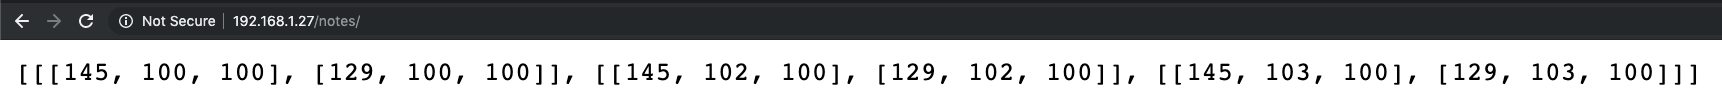
\includegraphics[width=\textwidth]{api}

Cały kod API to mapowanie URL do widoków oraz widoki, używające interface singletona, opisanego w poprzedniej sekcji.

\begin{lstlisting}[language=Python]
from . import views


route_handlers = [
    ('/notes/', 'GET', views.get_notes),
    ('/notes/', 'POST', views.set_notes)
]

...

from code.config import midi_messages


def get_notes(http_client, http_response):
    messages = midi_messages.slots.messages
    http_response.WriteResponseJSONOk(messages)


def set_notes(http_client, http_response):
    slots = http_client.ReadRequestContentAsJSON()
    for slot, messages in enumerate(slots):
        midi_messages.slots.set(slot, messages)
    midi_messages.save()
    http_response.WriteResponseOk()

\end{lstlisting}

\newpage
\section{Konfigurator}

\subsection{Interpretacja ustawień MIDI}

Można zauważyć, że ani nadajnik ani odbiornik w żaden sposób nie interpretują komunikatów MIDI. Te komponenty systemu nie mają pojęcia co one przesyłają, po prostu widzą, że mają sprawę z trzema bajtami. Natomiast po stronie konfiguratora te dane musimy przetłumaczyć na język ludzi. Poniżej jest przedstawiona część kodu GUI, wykonująca to zadanie.


\begin{lstlisting}[language=Python, breaklines=true]
MESSAGE_TYPES = {
    0b1001: 'note_on',
    0b1000: 'note_off',
    0b1010: 'polyphonic',
    0b1011: 'cc',
    0b1100: 'pc',
    0b1101: 'channel_pressure',
    0b1110: 'pitch_bend'
}
MESSAGE_TYPE_TO_BYTE = {v: k for k, v in MESSAGE_TYPES.items()}


class MidiMessage:

    def __init__(self, status, data_1=None, data_2=None):
        self.status = status
        self.data_1 = data_1
        self.data_2 = data_2

    @classmethod
    def from_form(cls, _type, channel=None, data_1=None, data_2=None):
        status = MESSAGE_TYPE_TO_BYTE[_type] * 2 ** 4 + int(channel)
        return cls(status, int(data_1), int(data_2))

    @property
    def type(self):
        type_byte = self.status // 2 ** 4
        return MESSAGE_TYPES[type_byte]

    @property
    def channel(self):
        channel_byte = self.status - (self.status // 2 ** 4) * 2 ** 4
        return channel_byte

    @property
    def raw(self):
        return [self.status, self.data_1, self.data_2]
\end{lstlisting}

\subsection{GUI}

GUI zostało napisane w frameworku Kivy. Poniżej są przedstawione przykładowe widgety do reprezentowania ustawień MIDI.

\begin{lstlisting}[language=Python, breaklines=true]
Spinner(text=message_type or '<Select>', values=MESSAGE_TYPES.values())
Spinner(text=str(channel) or '1', values=(str(i) for i in range(1, 17)))
TextInput(multiline=False, input_type='number', text=str(data_2))
Button(text='Delete')
\end{lstlisting}

Komunikacja z API jest realizowana przez biblioteke \textit{requests}.

\begin{lstlisting}[language=Python]
def get_slots():
    response = requests.get('http://192.168.1.27/notes/').text
    return json.loads(response)


def set_slots(slots):
    slots = [[m.raw for m in messages] for messages in slots]
    return requests.post('http://192.168.1.27/notes/', json=slots)
\end{lstlisting}

Przykładowa konfiguracja none\_on/note\_off per przycisk wygląda następująco:

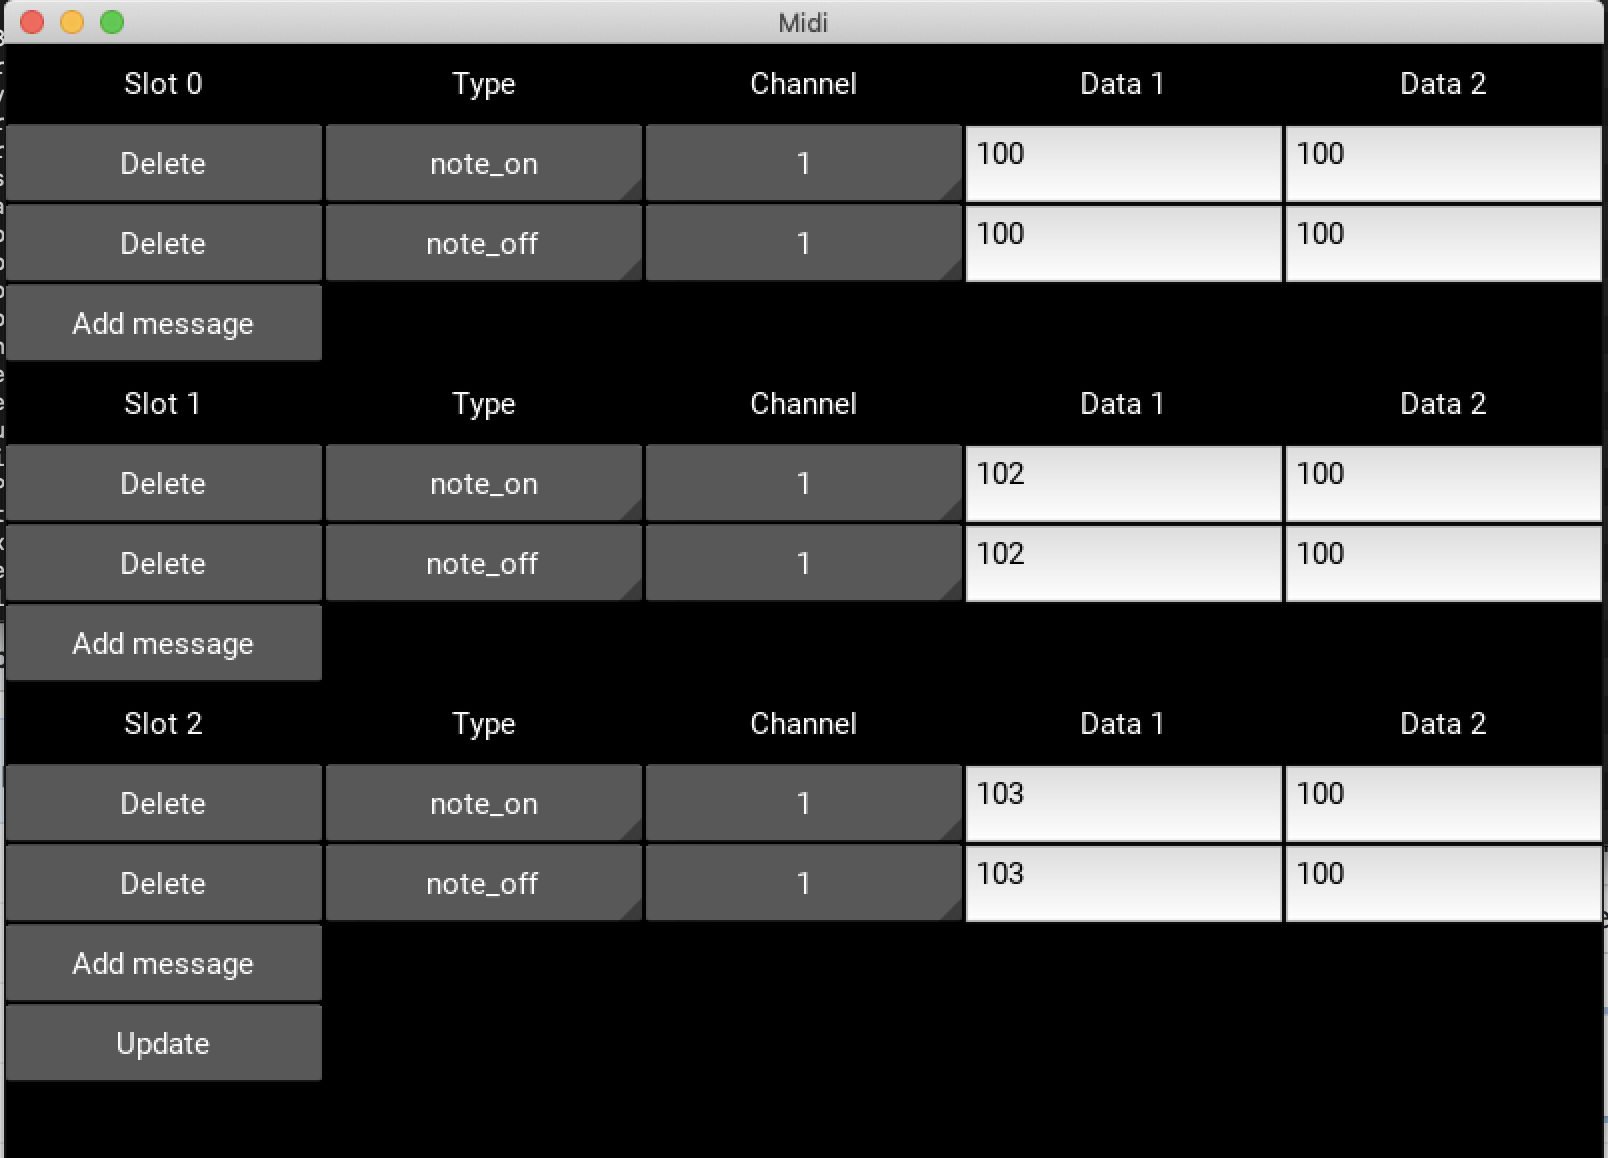
\includegraphics[width=\textwidth]{gui}

\subsection{Eksportowanie}

Kivy pozwala na eksportowanie aplikacji desktopowej oraz mobilnej. Zostało przetestowane eksportowanie dla systemu Mac OS. Wymaga zainstalowania biblioteki \textit{pyinstaller} oraz odpalenia komendy:
\begin{lstlisting}[language=bash, breaklines = true]
pyinstaller -y --clean --windowed --name touchtracer --exclude-module _tkinter --exclude-module Tkinter --exclude-module enchant --exclude-module twisted main.py
\end{lstlisting}

\section{Podsumowanie}

Projekt udało się zrealizować. Moduł HM-10 potrafi z zadowalającą szybkością przesyłać informację o wciśniętych przyciskach. Moduł ESP-32, zaprogramowany w języku MicroPython radzi sobie z jednoczesnym serwowaniem API, oraz komunikacją z modułem BLE i złączem MIDI poprzez UART.

Znane problemy:

\begin{itemize}
\item Bardzo trudno było znaleźć dokumentację do wykorzystanego klonu modułu HM-10. Większość komend trzeba było znajdować metodą prób i błędów. Problem można rozwiązać jedynie kupując droższy oryginalny moduł.
\item Proces parowania modułów BLE w tym projekcie jest uproszczony i ma wady. Nie ma żadnego sprawdzenia, czy zeskanowany moduł jest nadajnikiem, połączenie jest realizowane automatycznie z najbliższym modułem BLE w zasięgu odbiornika. Żeby ten problem rozwiązać można by było dodać przycisk na odbiorniku oraz skonfigurować jeden z przycisków na nadajniku tak, żeby parowanie się odbywało tylko przy wciśnięciu obu przycisków jednocześnie. Alternatywnie można sprawdzać adres MAC zeskanowanego urządzenia.
\item Nie ma możliwości zmiany ustawień punktu dostępu z poziomu użytkownika.
\item Czasami nadajnik traci połączenie z odbiornikiem. Żeby tego uniknąć zaleca się podpinać kilka baterii CR2032 równolegle.
\item Czasami nie działa automatyczny reconnect w przypadku wyłączenia nadajnika. W takim przypadku jedynym rozwiązaniem jest restartowanie odbiornika.
\end{itemize}

Kod projektu:

\href{https://github.com/alexpilk/esp32-wireless-midi}{https://github.com/alexpilk/esp32-wireless-midi}.
\bigbreak

Na tym filmie odbiornik jest podłączony przez złącze MIDI do karty dźwiękowej. Sygnał z wejścia jest odbierany przez program Reaper, a nuty MIDI są przepuszczane przez syntezator:

\href{https://youtu.be/\_9DkzAXo7i8}{https://youtu.be/\_9DkzAXo7i8}
\bigbreak

Na tym filmie odbiornik jest podłączony przez złącze MIDI do wzmacniacza Kemper Profiling Amplifier. Poprzez komunikaty typu \textit{Control Change} są zdalnie prełączane presety:

\href{https://youtu.be/wr5JzCO7T9I}{https://youtu.be/wr5JzCO7T9I}
\bigbreak

Poniżej są przedstawione zdjęcia nadajnika i odbiornika:


\begin{center}
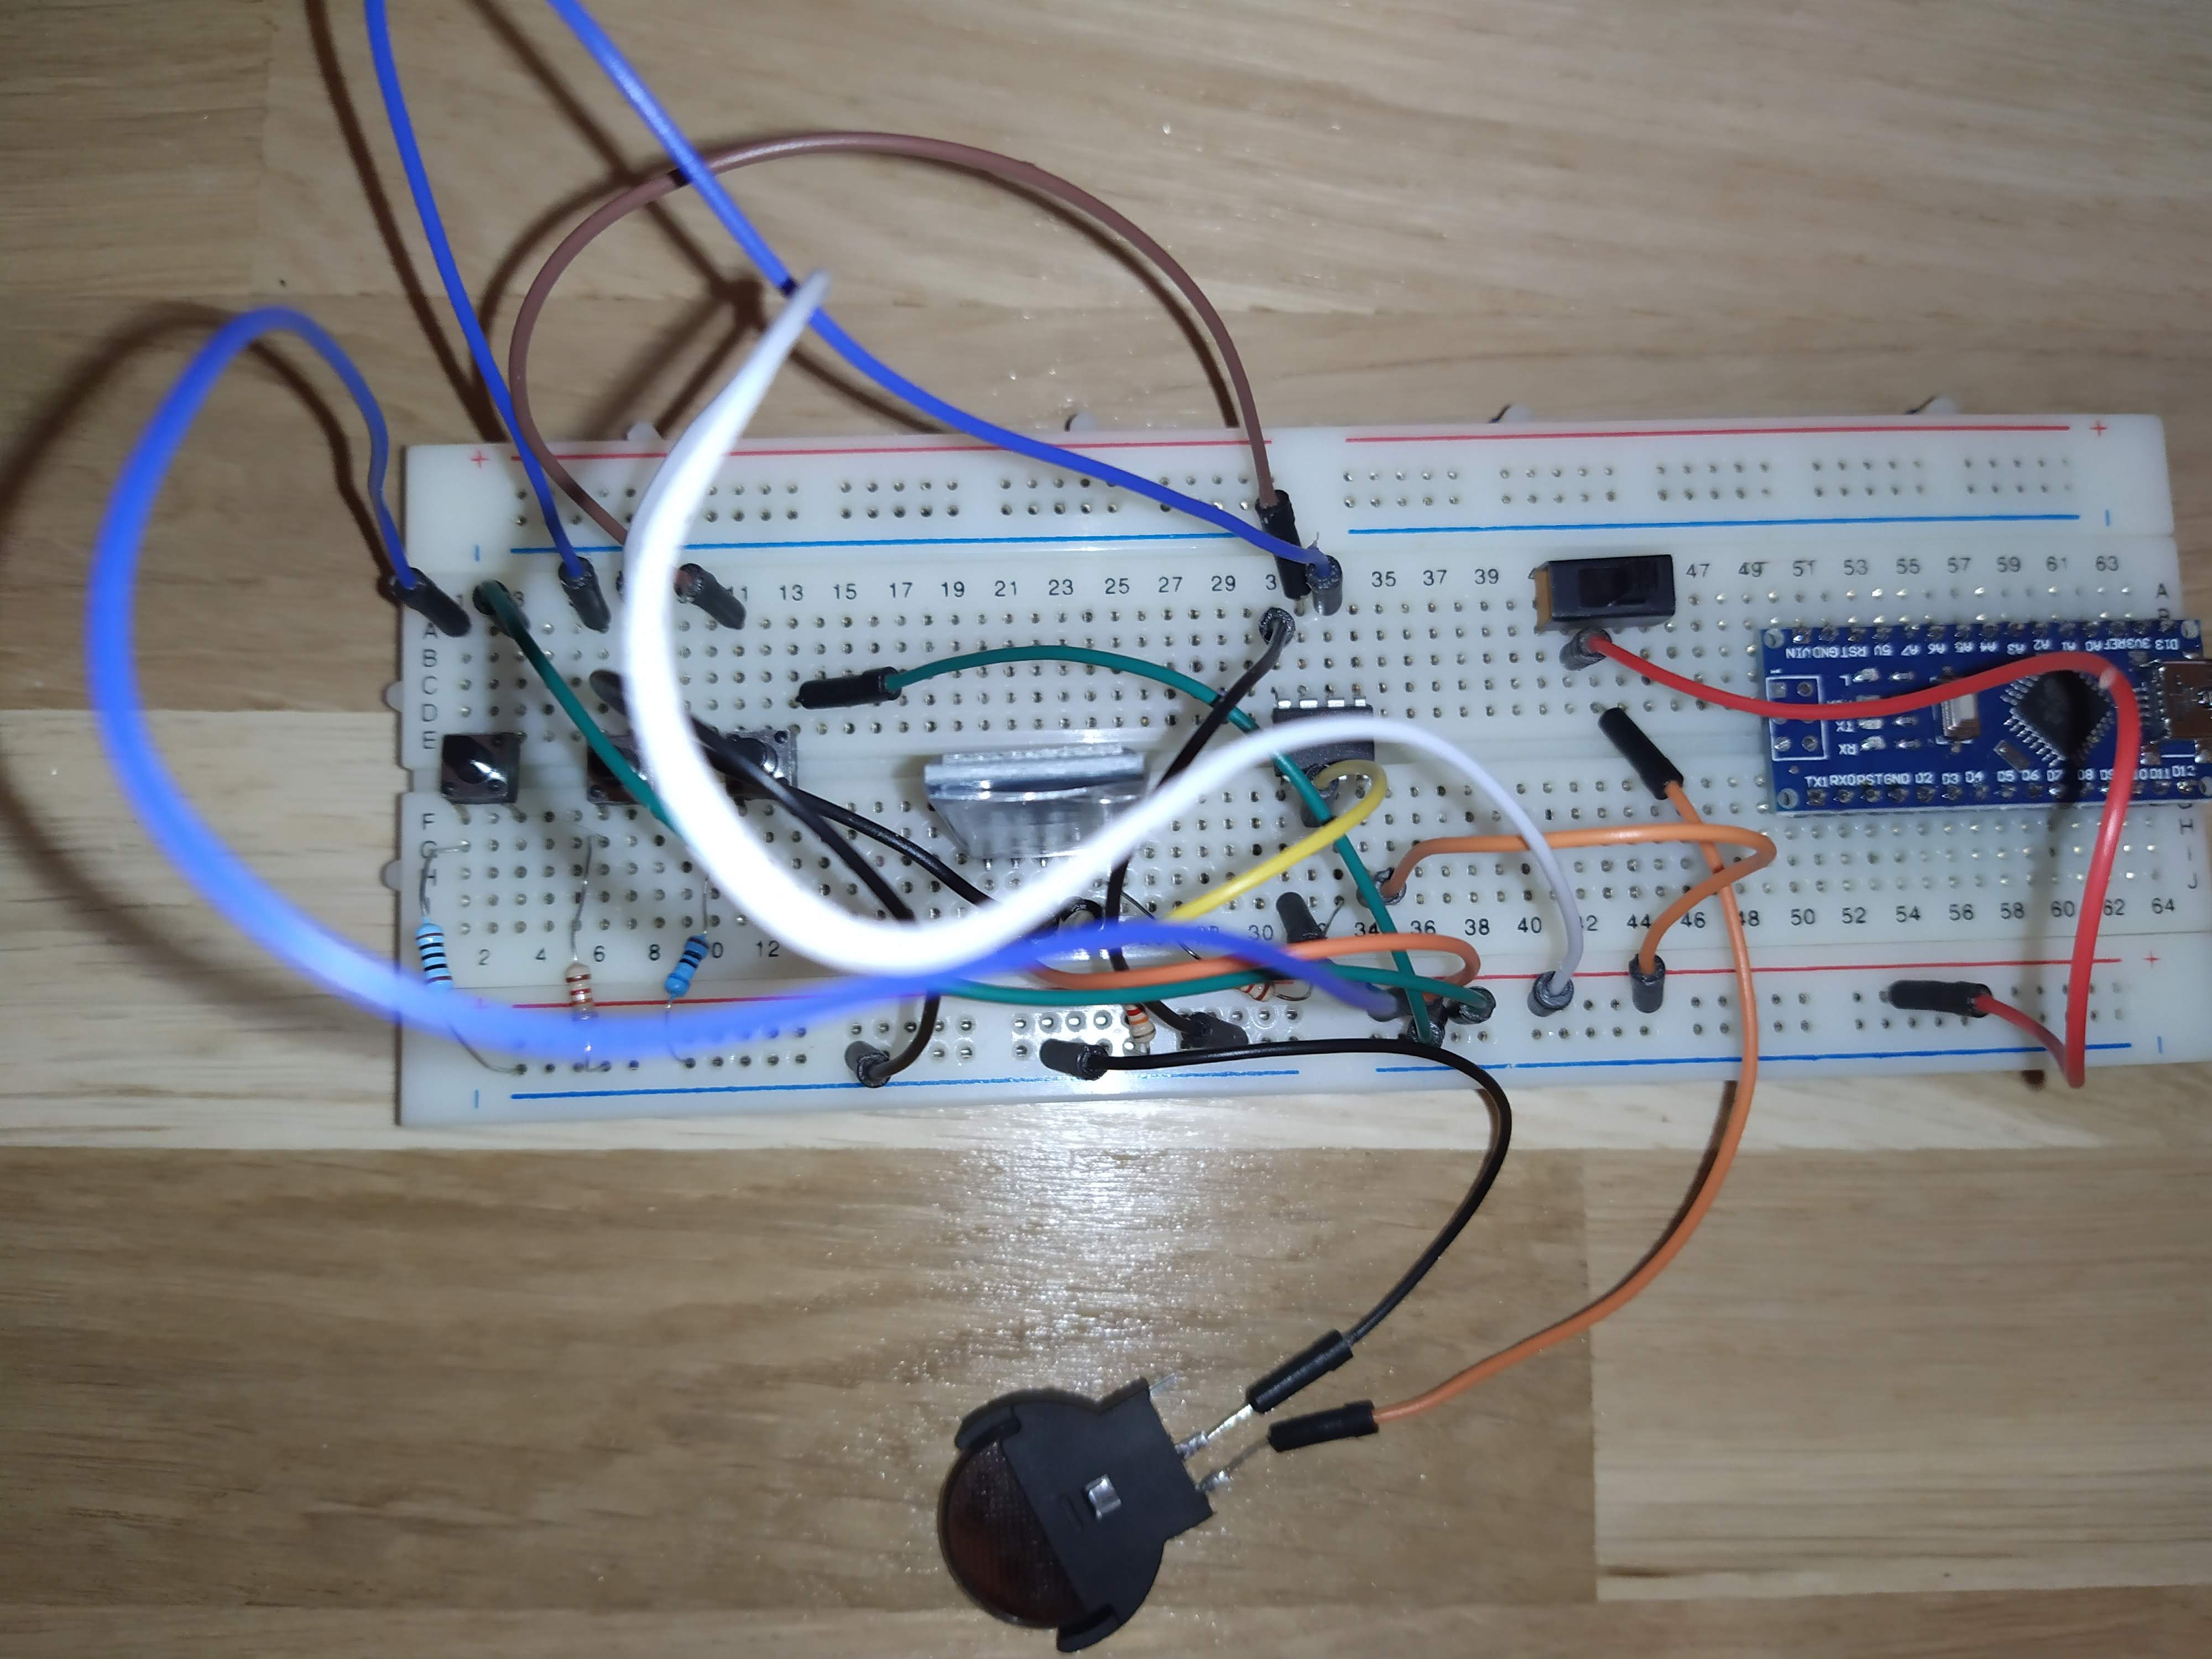
\includegraphics[width=\textwidth]{nadajnik-1}
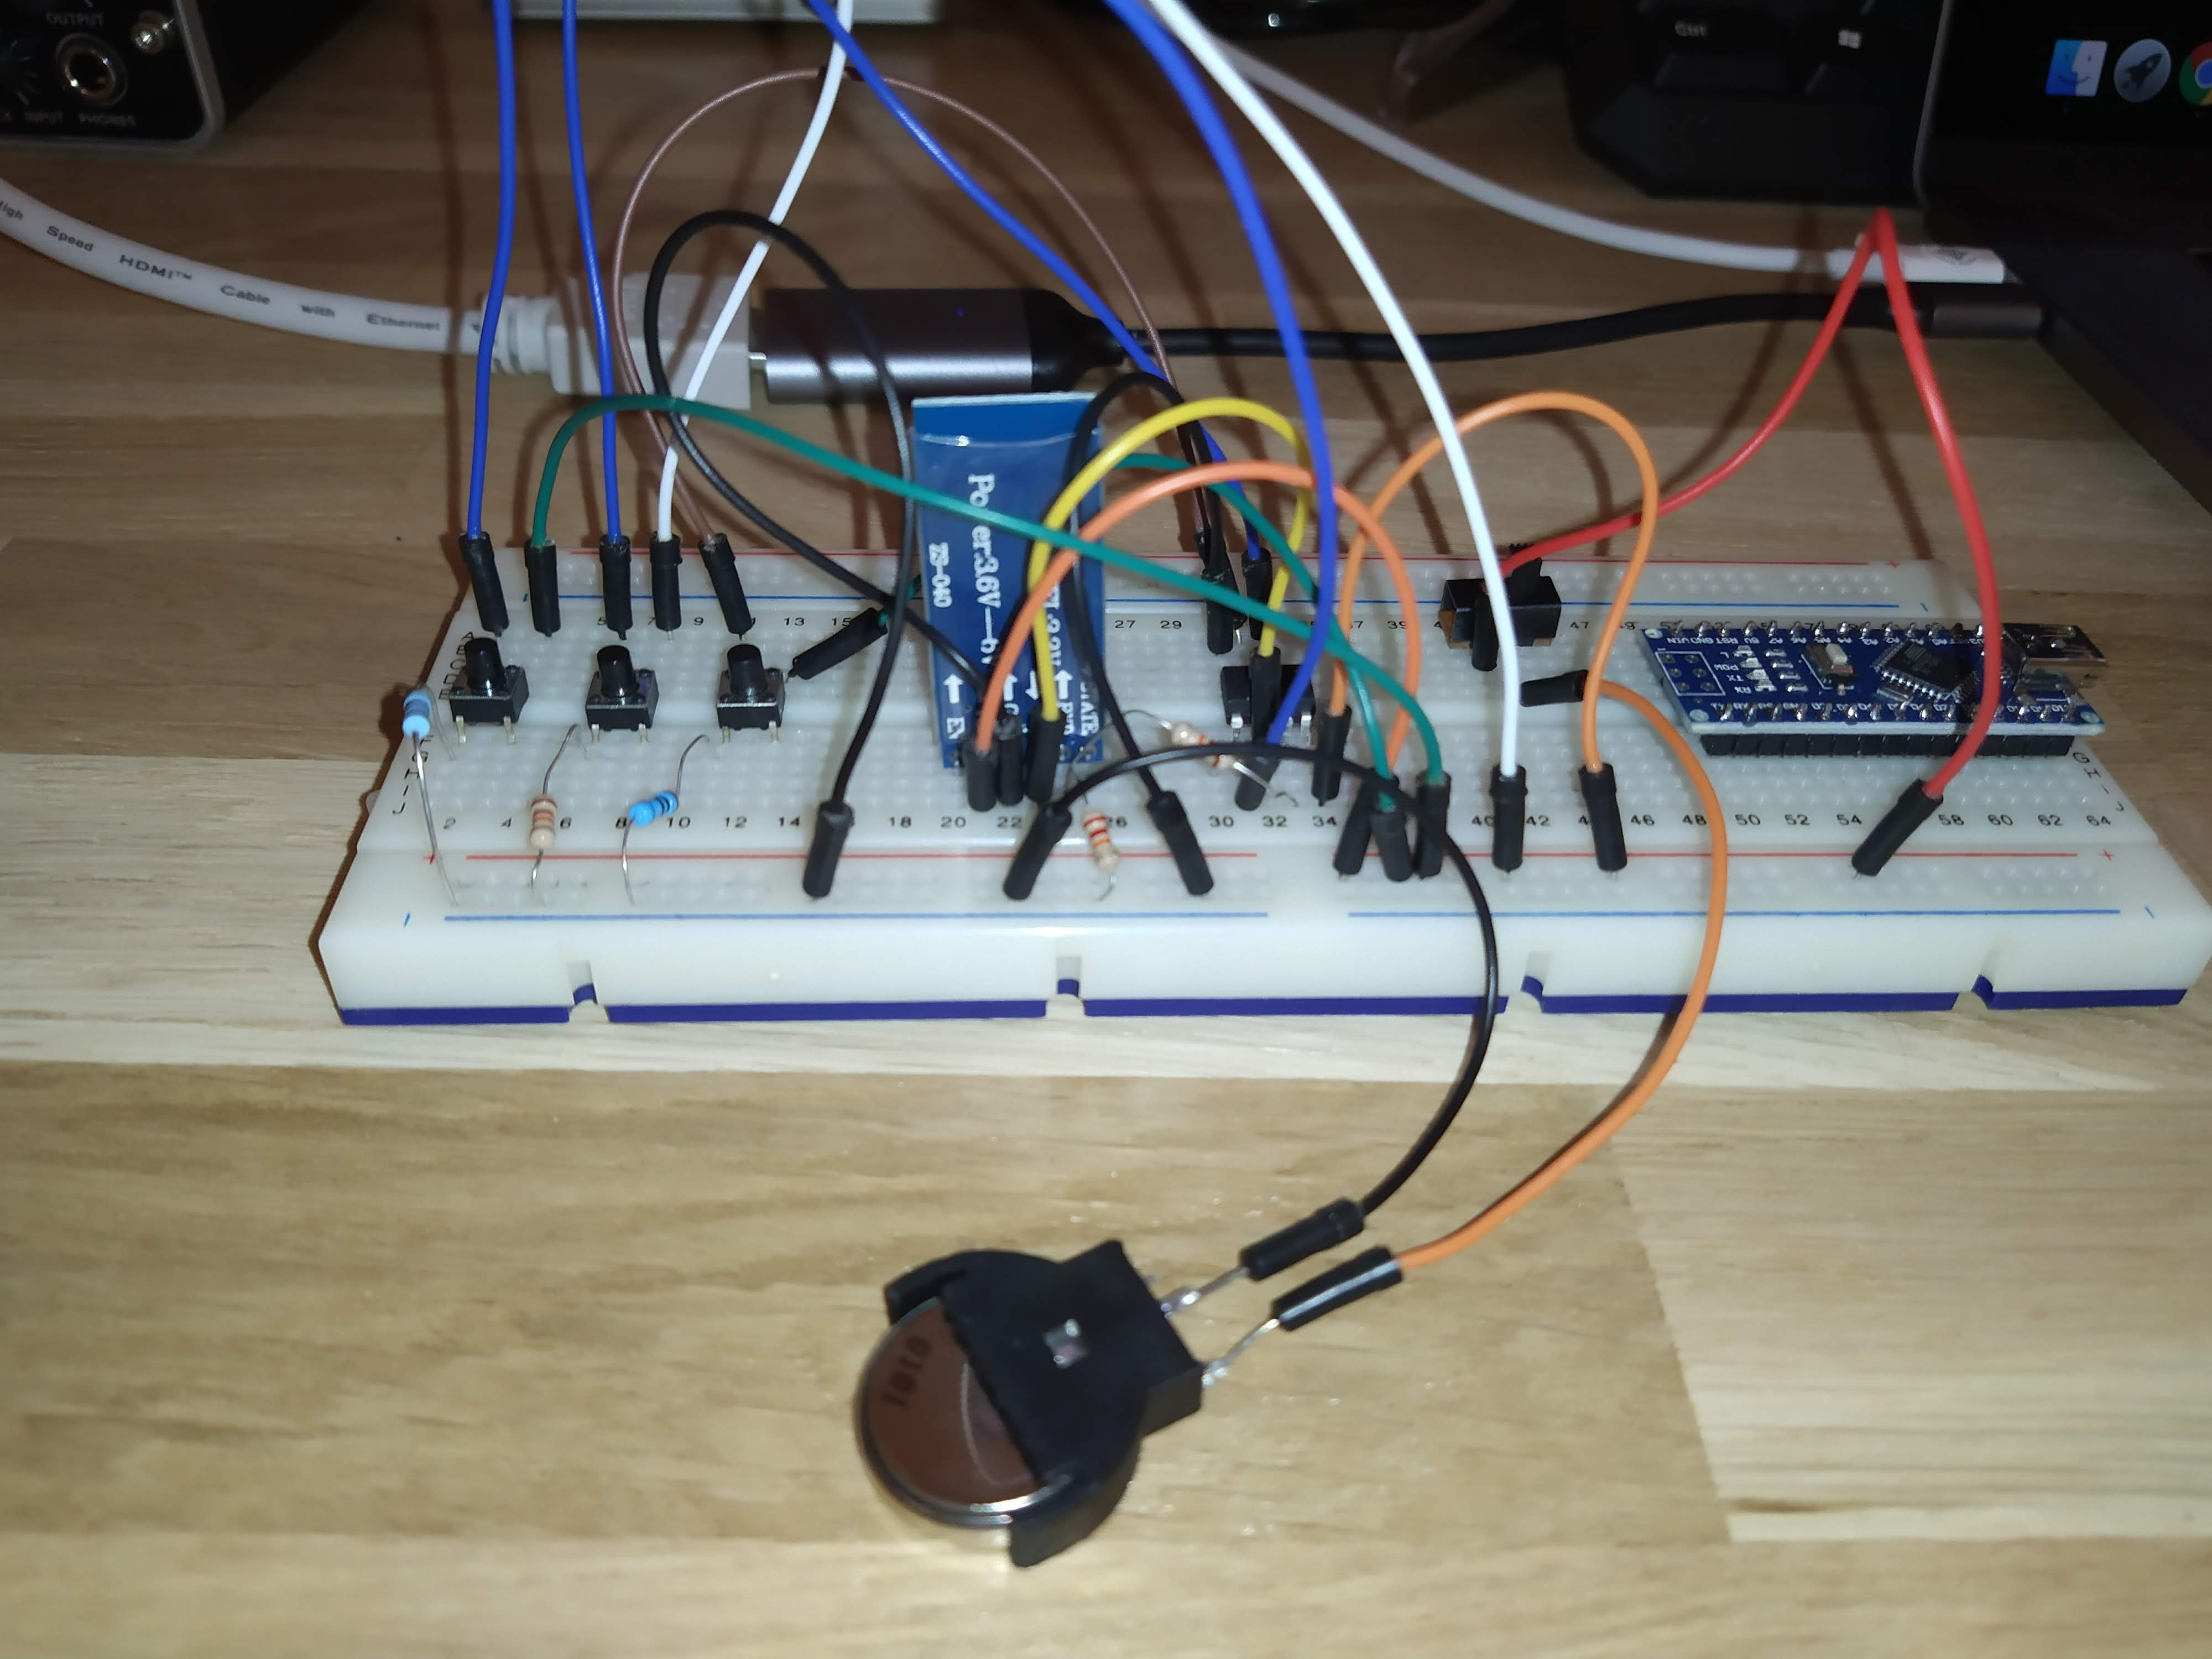
\includegraphics[width=\textwidth]{nadajnik-2}
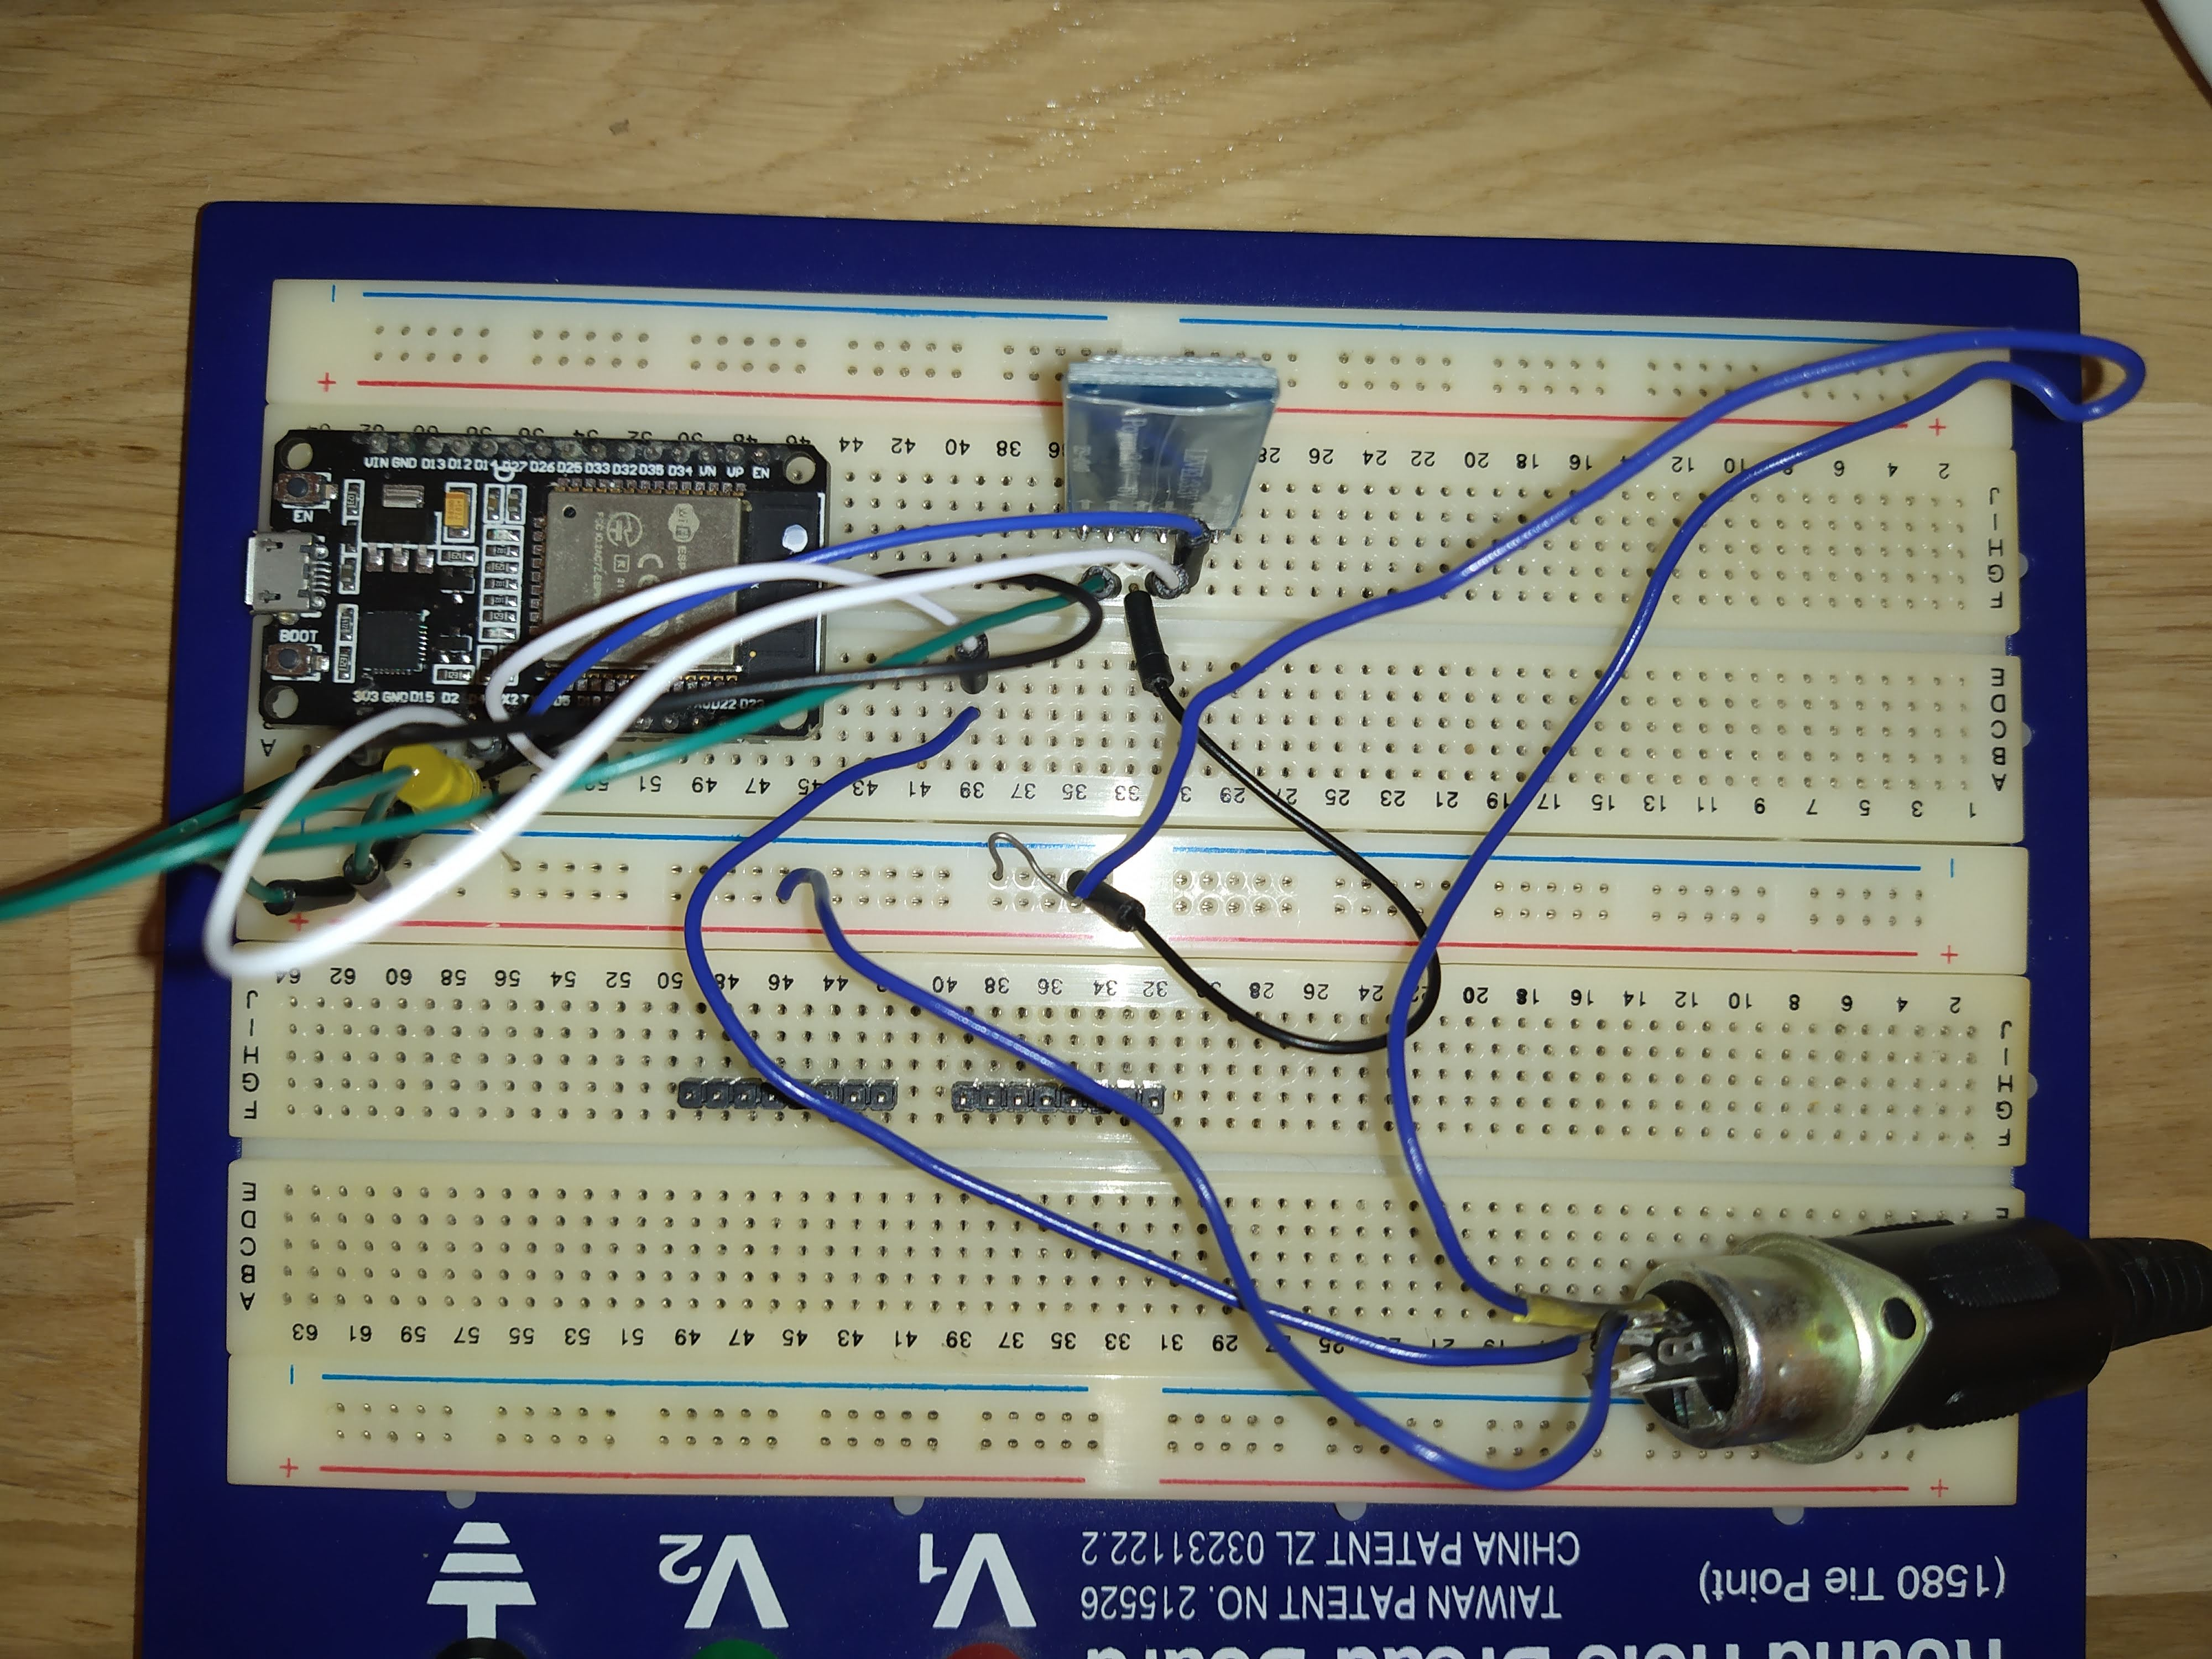
\includegraphics[width=\textwidth]{odbiornik-1}
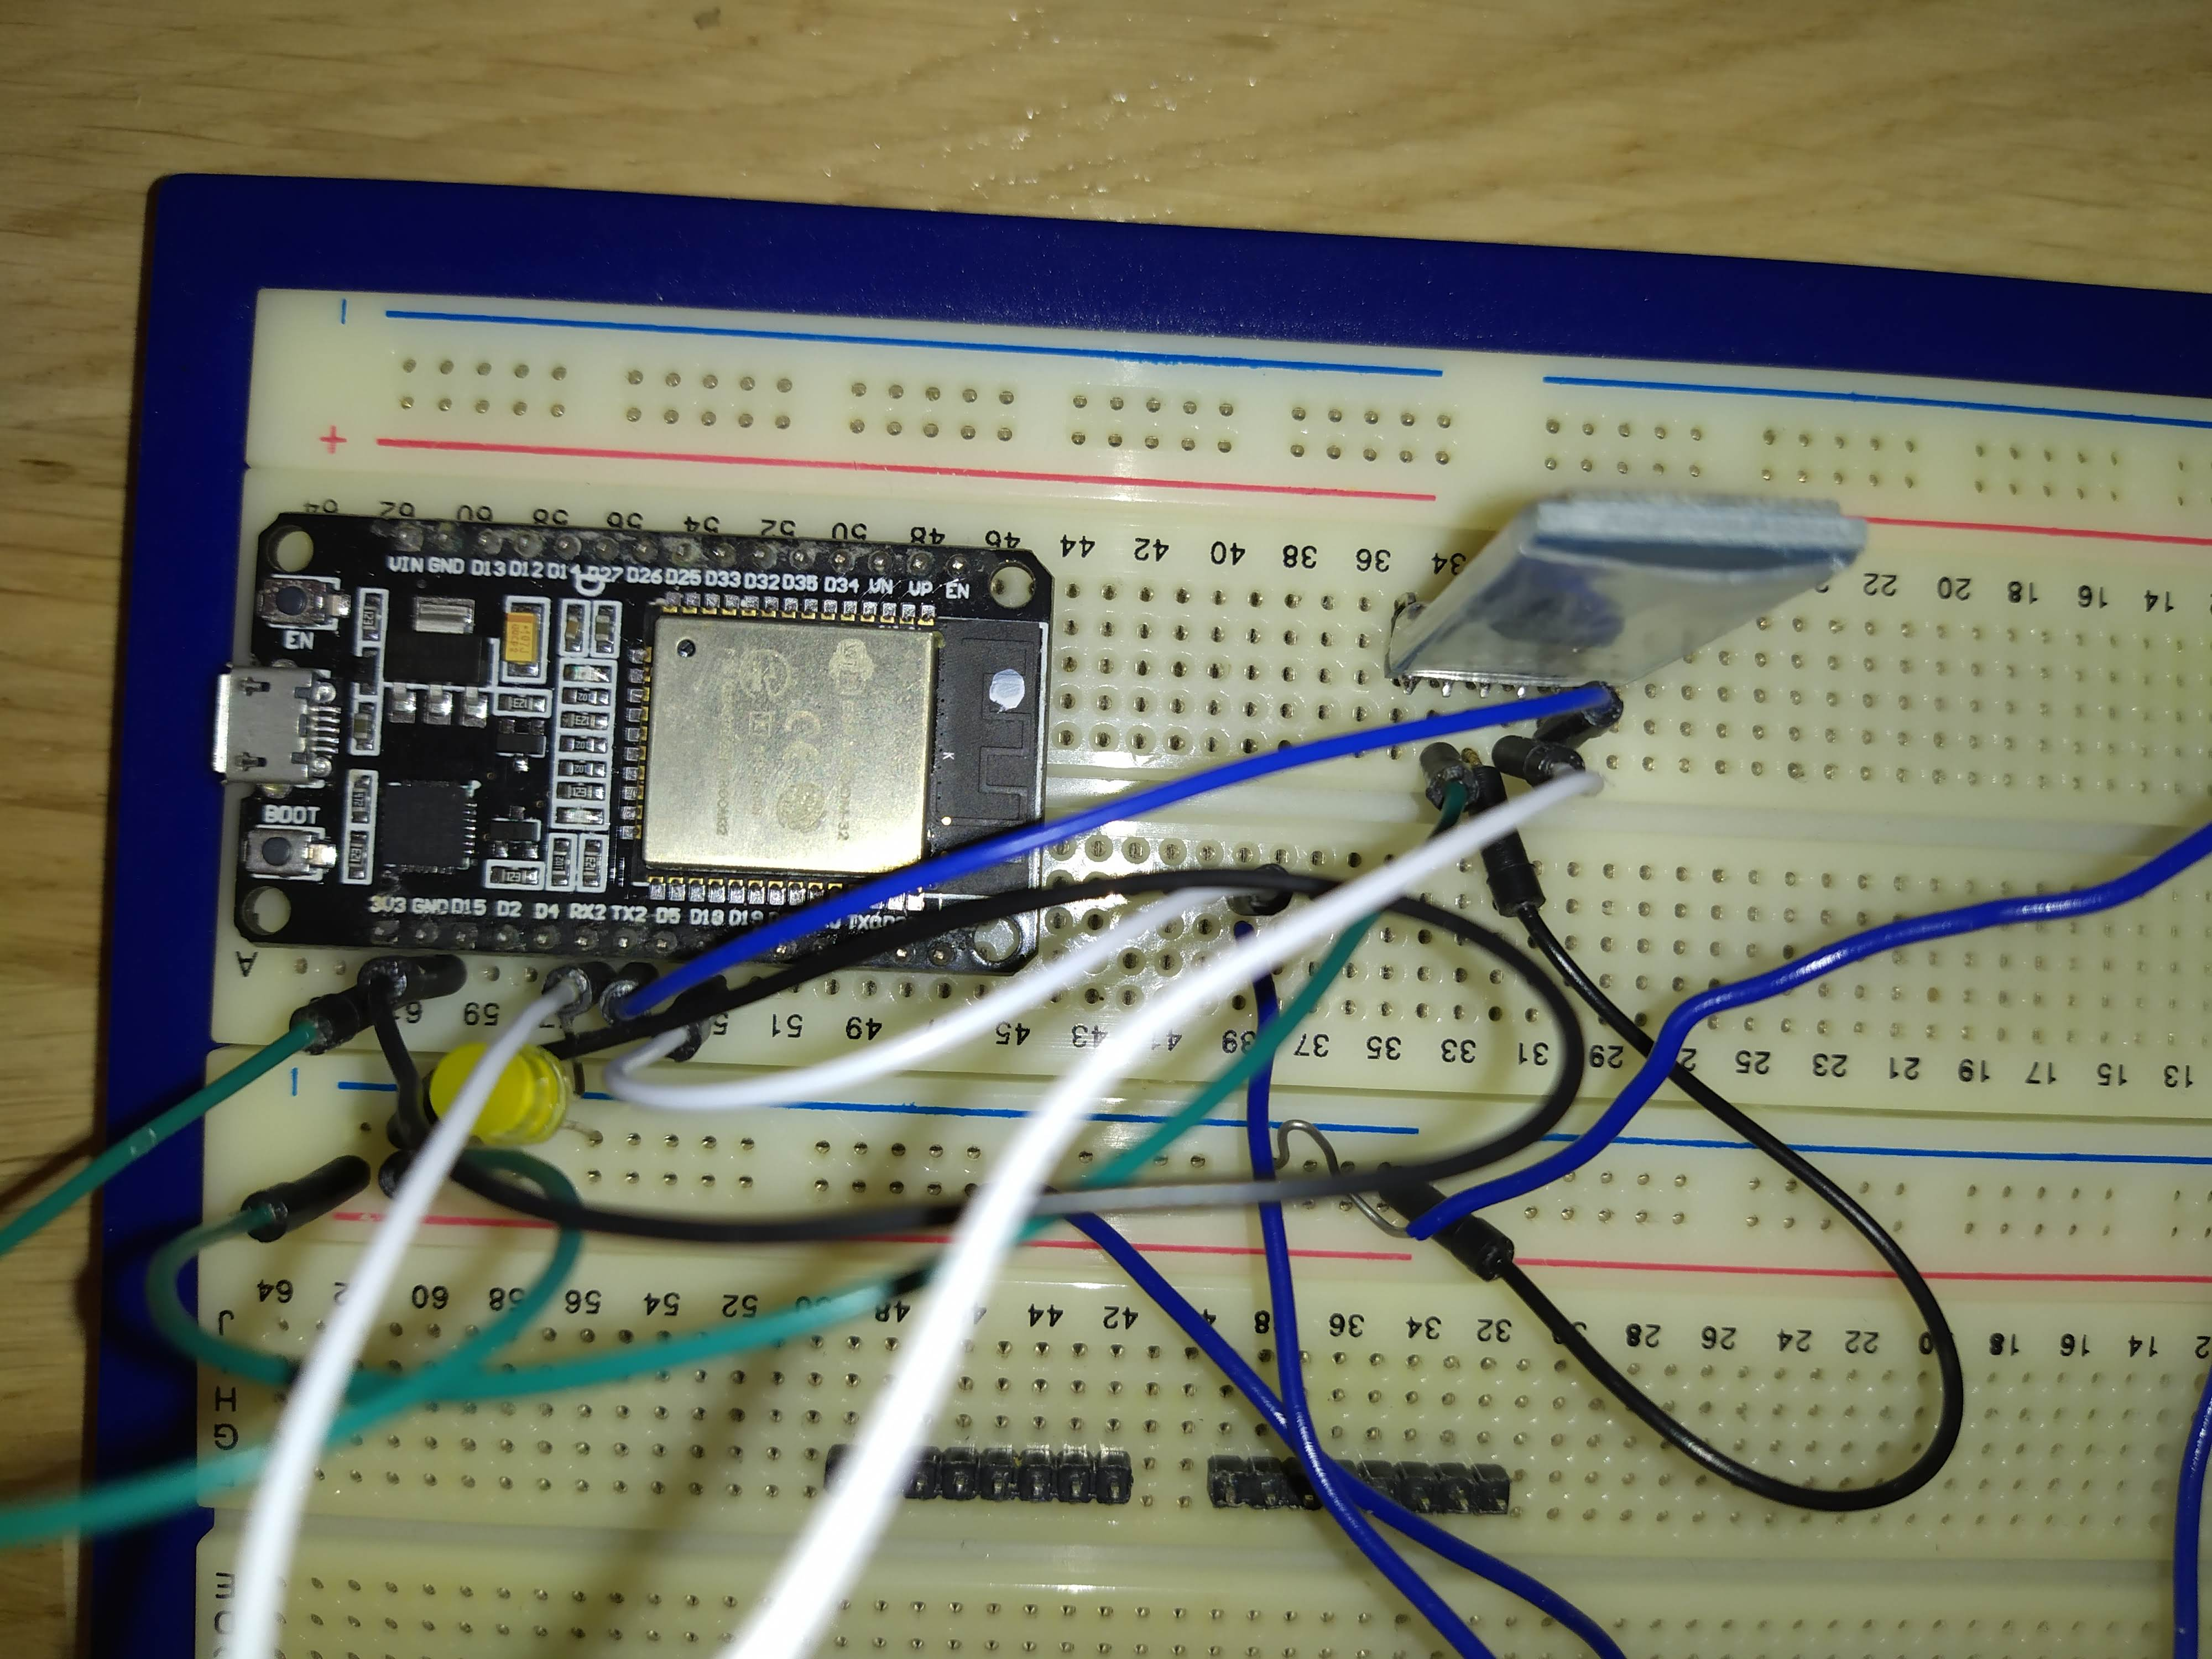
\includegraphics[width=\textwidth]{odbiornik-2}
\end{center}


\addcontentsline{toc}{chapter}{\bibname} %utworzenie w spisie treści pozycji Literatura
% \bibliography{bibliografia} % wstawia bibliografię korzystając z pliku bibliografia.bib - dotyczy BibTeXa, jeżeli nie korzystamy z BibTeXa należy użyć otoczenia 

\begin{thebibliography}{9}

\bibitem{}
\href{http://docs.micropython.org/en/v1.11/}{Dokumentacja języka MicroPython}

\bibitem{}
\href{https://www.arduino.cc/en/Reference/softwareSerial}{Dokumentacja biblioteki SoftwareSerial}

\bibitem{}
\href{https://www.arduino.cc/en/tutorial/debounce}{Poradnik do debounce-owania przycisków na Arduino}

\bibitem{}
\href{https://www.arduino.cc/en/Hacking/LibraryTutorial}{Poradnik do tworzenia własnych bibliotek Arduino}

\bibitem{}
\href{https://circuits4you.com/2018/12/31/esp32-devkit-esp32-wroom-gpio-pinout/}{Pinout płyty ESP-32}

\bibitem{}
\href{https://components101.com/microcontroller/attiny85-pinout-datasheet}{Pinout i specyfikacja ATTINY85}

\bibitem{}
\href{https://www.midi.org/specifications-old/item/table-1-summary-of-midi-message}{Specyfikacja komunikatów MIDI}

\bibitem{}
\href{https://www.midi.org/articles-old/updated-how-to-make-your-own-3-5mm-mini-stereo-trs-to-midi-5-pin-din-cables}{Specyfikacja złącza DIN-5 dla MIDI}

\bibitem{}
\href{https://www.instructables.com/id/Arduino-Nano-as-Attiny-85-programmer-and-5-LED-POV/}{Poradnik do programowania ATTINY85 przez Arduino Nano}

\bibitem{}
\href{https://kivy.org/doc/stable-1.11.0/api-kivy.html}{Dokumentacja frameworku Kivy}

\bibitem{}
\href{https://github.com/jczic/MicroWebSrv}{Dokumentacja frameworku MicroWebSrv}

\bibitem{}
\href{http://denethor.wlu.ca/arduino/MLT-BT05-AT-commands-TRANSLATED.pdf}{Komendy AT dla modułu HM-10 MLT-BT05}

\end{thebibliography}

%opcjonalnie może się tu pojawić spis rysunków i tabel
% \listoffigures
% \listoftables
\end{document}
